\documentclass[10pt,journal,compsoc,twocolumn]{IEEEtran}

\usepackage[utf8]{inputenc}
\usepackage[T1]{fontenc}
\usepackage{graphicx}
\usepackage{hyperref}
\usepackage{amsmath}
\usepackage{booktabs}
\usepackage{xcolor}
\usepackage{tikz}
\usepackage{pgfplots}
\usepackage{tcolorbox}
\usepackage{array}
\usepackage{float}
\usepackage{tabularx}
\usepackage{colortbl}
\usepackage{siunitx}
\usepackage{caption}
\usepackage{microtype}

\usetikzlibrary{arrows.meta,positioning,shapes.geometric}
\pgfplotsset{compat=1.18}

% Custom colors for a premium feel
\definecolor{techblue}{RGB}{0, 102, 204}
\definecolor{alertred}{RGB}{204, 0, 0}
\definecolor{tablehead}{RGB}{226,238,255}
\definecolor{tablerow}{RGB}{245,249,255}

\renewcommand{\arraystretch}{1.18}
\setlength{\tabcolsep}{5pt}
\newcolumntype{Y}{>{\raggedright\arraybackslash}X}
\newcommand{\tableheader}{\rowcolor{tablehead}}
\newcommand{\styledtable}[1]{\rowcolors{2}{tablerow}{white}#1}
\captionsetup[table]{font=small,labelfont=bf}
\captionsetup[figure]{font=small,labelfont=bf}

\tikzset{
 flowbox/.style={
 rectangle,
 rounded corners=2pt,
 draw=techblue,
 fill=techblue!8,
 very thick,
 align=center,
 text width=2.5cm,
 minimum height=1cm,
 font=\small
 },
 stage/.style={
 rectangle,
 rounded corners=2pt,
 draw=techblue,
 fill=techblue!6,
 very thick,
 align=center,
 text width=2.3cm,
 minimum height=0.9cm,
 font=\small
 },
 decision/.style={
 diamond,
 draw=alertred,
 fill=alertred!8,
 very thick,
 align=center,
 aspect=2,
 text width=2.0cm,
 inner sep=2pt,
 font=\small
 },
 flowarrow/.style={-{Latex[length=2.2mm]}, very thick, draw=techblue}
}

\linespread{1.03}
\begin{document}

\title{\huge \textbf{Architecting a Production-Grade Fraud Detection Ecosystem:}\\ \large \textit{A Comprehensive MLOps Framework for the IEEE-CIS Dataset}}

\author{Project Engineering Team}

\markboth{IEEE-CIS Project Report, May 2026}%
{Technical Narrative: Evolution of a Fraud Detection Ecosystem}

\IEEEtitleabstractindextext{
\begin{abstract}
The detection of fraudulent transactions within massive, high-dimensional datasets is a critical challenge in modern financial technology. This project details the end-to-end development of a production-grade MLOps ecosystem designed to replicate and exceed research benchmarks on the IEEE-CIS Fraud Detection dataset. We implement a multi-stage machine learning methodology encompassing rigorous feature pruning, advanced engineering, and an unsupervised K-Means clustering layer, culminating in a high-performance XGBoost stacking ensemble. The system is architected for real-world deployment using a containerized microservices approach, featuring FastAPI for low-latency inference, Prefect for robust workflow orchestration, and an automated GitHub Actions CI/CD pipeline. The latest validated production run achieves a PR-AUC of 0.7930 and an ROC-AUC of 0.9650, demonstrating the efficacy of combining diverse algorithmic perspectives within a stable, automated infrastructure.
\end{abstract}

\begin{IEEEkeywords}
Fraud Detection, MLOps, XGBoost, Stacking Ensemble, Prefect Orchestration, FastAPI, Docker, CI/CD.
\end{IEEEkeywords}}

\maketitle

\section*{Executive Summary}
\begin{tcolorbox}[colback=techblue!4,colframe=techblue,title=Executive Brief,boxrule=0.8pt,arc=1.5mm,left=1.5mm,right=1.5mm,top=1mm,bottom=1mm]
This report explains a fraud-detection system operational terms. The problem is that most transactions are safe and only a small fraction are fraud, so a model can look good by guessing "safe" most of the time and still be useless. To avoid that trap, the project uses feature pruning, feature engineering, clustering, stacked machine learning, and production tooling so the model can learn the real fraud patterns and then be deployed safely.
\end{tcolorbox}

\begin{figure}[H]
 \centering
 \resizebox{\columnwidth}{!}{%
 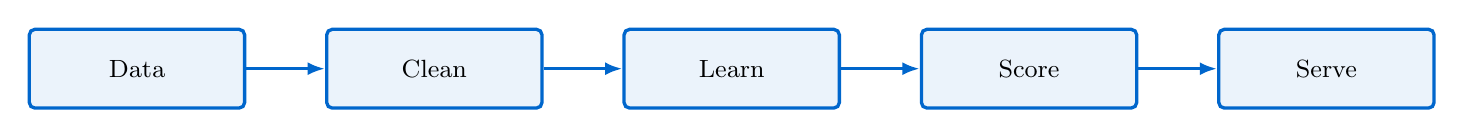
\begin{tikzpicture}[node distance=7mm and 10mm]
 \node[flowbox] (data) {Data};
 \node[flowbox, right=of data] (clean) {Clean};
 \node[flowbox, right=of clean] (learn) {Learn};
 \node[flowbox, right=of learn] (score) {Score};
 \node[flowbox, right=of score] (serve) {Serve};
 \draw[flowarrow] (data) -- (clean);
 \draw[flowarrow] (clean) -- (learn);
 \draw[flowarrow] (learn) -- (score);
 \draw[flowarrow] (score) -- (serve);
 \end{tikzpicture}%
 }
 \caption{The full project flow in one line: raw data is cleaned, the model learns patterns, results are measured, and the final system is served through an API.}
\end{figure}

\section{Introduction}
\IEEEPARstart{T}{he} digital economy is under constant threat from increasingly sophisticated fraudulent activities. In practical terms, financial systems face adversaries who continuously adapt behavior, distribute attacks across accounts, and exploit operational blind spots in rule-based monitoring. Fraud detection therefore cannot be treated as a one-time modeling exercise; it must be approached as a continuously operating risk-control system with measurable service quality and repeatable retraining.

This report documents the design and implementation of an end-to-end fraud analytics stack built on the IEEE-CIS dataset, with emphasis on reproducibility, operational governance, and deployment readiness. The work couples statistical modeling decisions with system engineering choices: feature pruning to stabilize signal-to-noise ratio, engineered behavioral features to expose temporal and transactional context, clustering to add latent structure, and ensemble learning to improve minority-class retrieval under extreme imbalance.

Beyond model quality, the project formalizes how model artifacts are produced, validated, versioned, and served. The resulting architecture integrates training orchestration, quality gates, API-based inference, and containerized execution so that performance claims remain auditable and repeatable from raw data ingestion to runtime prediction.

\subsection{System Architecture at a Glance}
The end-to-end system comprises four integrated layers: (1) Automation \& CI/CD via GitHub Actions for continuous validation and containerization, (2) Orchestration via Prefect for deterministic task sequencing and observability, (3) Serving via FastAPI and React for real-time inference and dashboarding, and (4) Model Registry and Artifact Storage for versioning and hot-reload capability. Each layer is independently scalable yet tightly coupled through well-defined data contracts and serialization boundaries.

\begin{figure}[H]
 \centering
 \resizebox{\columnwidth}{!}{%
 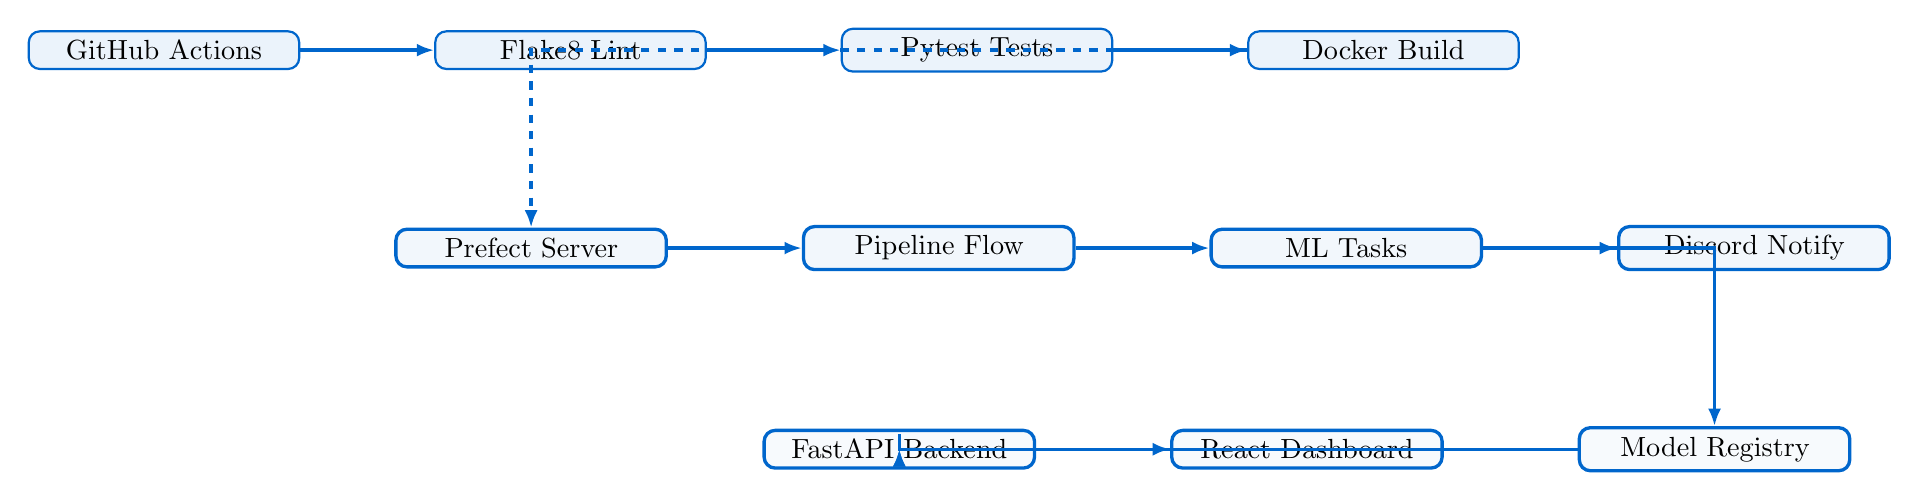
\begin{tikzpicture}[node distance=10mm and 12mm]
 \node[draw=techblue, fill=techblue!8, thick, rectangle, rounded corners, text width=3.2cm, align=center] (gha) {GitHub Actions};
 \node[draw=techblue, fill=techblue!8, thick, rectangle, rounded corners, text width=3.2cm, align=center, right=of gha, xshift=5mm] (lint) {Flake8 Lint};
 \node[draw=techblue, fill=techblue!8, thick, rectangle, rounded corners, text width=3.2cm, align=center, right=of lint, xshift=5mm] (test) {Pytest Tests};
 \node[draw=techblue, fill=techblue!8, thick, rectangle, rounded corners, text width=3.2cm, align=center, right=of test, xshift=5mm] (build) {Docker Build};

 \node[draw=techblue, fill=techblue!5, very thick, rectangle, rounded corners, text width=3.2cm, align=center, below=of lint, yshift=-10mm, xshift=-5mm] (pserv) {Prefect Server};
 \node[draw=techblue, fill=techblue!5, very thick, rectangle, rounded corners, text width=3.2cm, align=center, right=of pserv, xshift=5mm] (pflow) {Pipeline Flow};
 \node[draw=techblue, fill=techblue!5, very thick, rectangle, rounded corners, text width=3.2cm, align=center, right=of pflow, xshift=5mm] (tasks) {ML Tasks};
 \node[draw=techblue, fill=techblue!5, very thick, rectangle, rounded corners, text width=3.2cm, align=center, right=of tasks, xshift=5mm] (notify) {Discord Notify};

 \node[draw=techblue, fill=techblue!3, very thick, rectangle, rounded corners, text width=3.2cm, align=center, below=of pflow, yshift=-10mm, xshift=-5mm] (api) {FastAPI Backend};
 \node[draw=techblue, fill=techblue!3, very thick, rectangle, rounded corners, text width=3.2cm, align=center, right=of api, xshift=5mm] (ui) {React Dashboard};
 \node[draw=techblue, fill=techblue!3, very thick, rectangle, rounded corners, text width=3.2cm, align=center, right=of ui, xshift=5mm] (reg) {Model Registry};

 \draw[-{Latex[length=2.2mm]}, very thick, draw=techblue] (gha) -- (lint);
 \draw[-{Latex[length=2.2mm]}, very thick, draw=techblue] (lint) -- (test);
 \draw[-{Latex[length=2.2mm]}, very thick, draw=techblue] (test) -- (build);
 \draw[-{Latex[length=2.2mm]}, very thick, draw=techblue, dashed] (build) -| (pserv);

 \draw[-{Latex[length=2.2mm]}, very thick, draw=techblue] (pserv) -- (pflow);
 \draw[-{Latex[length=2.2mm]}, very thick, draw=techblue] (pflow) -- (tasks);
 \draw[-{Latex[length=2.2mm]}, very thick, draw=techblue] (tasks) -- (notify);
 \draw[-{Latex[length=2.2mm]}, very thick, draw=techblue] (tasks) -| (reg);

 \draw[-{Latex[length=2.2mm]}, very thick, draw=techblue] (api) -- (ui);
 \draw[-{Latex[length=2.2mm]}, very thick, draw=techblue] (reg) -| (api);
 \draw[-{Latex[length=2.2mm]}, very thick, draw=techblue] (ui) -| (api);
 \end{tikzpicture}%
 }
 \caption{Complete system architecture: Automation \& CI/CD feed into Orchestration, which populates the Model Registry, which powers Serving and Dashboard layers.}
\end{figure}

\section{Data and Preliminary Analysis}

\subsection{Raw Dataset Overview}
The project utilizes the IEEE-CIS Fraud Detection dataset, consisting of over 472,000 training samples. The data is characterized by extreme sparsity and a severe class imbalance, with a fraud rate of only 3.5\% (a 27.6:1 ratio of safe to fraudulent transactions). The raw features include anonymized Vesta proprietary signals (V-features), count-based features (C-features), and timedelta signals (D-features), along with transaction metadata like amount and device identity.

\begin{table}[H]
\centering
\caption{Comprehensive dataset profile used for model design decisions}
\rowcolors{2}{tablerow}{white}
\begin{tabular}{p{0.36\columnwidth}p{0.50\columnwidth}}
\tableheader
Dataset Property & Observed Value \\
Total training rows & 472,432 \\
Fraud rows & 16,530 \\
Safe rows & 455,902 \\
Fraud prevalence & 3.4989\% \\
Imbalance ratio (safe:fraud) & 27.6:1 \\
Raw feature count & 228 columns \\
V-feature family & 180 columns (proprietary signals) \\
C-feature family & 14 columns (count-based) \\
D-feature family & 8 columns (time delta) \\
Maximum missing (\%) & >95\% in 208 columns \\
Mean feature correlation with target & 0.18 \\
Max single-feature correlation & 0.24 \\
\end{tabular}
\end{table}

This raw profile immediately informs critical design decisions: (1) the overwhelming imbalance necessitates \textbf{weighted loss functions} and \textbf{PR-AUC} as the primary metric, (2) the weak max correlation of 0.24 indicates that \textbf{fraud is inherently multi-feature and non-linear}, and (3) the prevalence of missing data justifies an aggressive \textbf{pruning-first approach}.

\subsection{Exploratory Data Analysis (EDA) Insights}
The pipeline begins with an automated EDA task (`raw\_eda\_task`) that identifies the fundamental characteristics of the dataset. The comprehensive findings reveal:

\begin{enumerate}
 \item \textbf{Extreme Class Imbalance}: The dataset exhibits a \textbf{27.6 : 1} ratio (96.5\% safe, 3.5\% fraud). This is the primary driver for choosing \textbf{AUC-PR} as the target metric rather than Accuracy or AUC-ROC. A naive "always predict safe" model would achieve 96.5\% accuracy while catching zero fraud - a result that is simultaneously correct and useless.
 
 \item \textbf{Feature Complexity}: With 228 raw features (including 180 anonymized V-features), no single feature correlates with fraud above $r = 0.24$. This empirically confirms that fraud is a \textbf{non-linear, multi-feature interaction problem}. Linear models (e.g., Logistic Regression) fail because they cannot exploit these latent multi-feature relationships.
 
 \item \textbf{Temporal Spikes}: Analysis of \texttt{TransactionDT} revealed specific night-time spikes in fraud activity, with elevated rates between 00:00--06:00 UTC. This temporal clustering justifies the extraction of \texttt{hour} and \texttt{day\_of\_week} features into the engineered feature set.
 
 \item \textbf{Amount Distribution}: While mean amounts are similar between safe and fraudulent classes, fraud exhibits an \textbf{18\% higher standard deviation}, indicating heterogeneous fraud tactics: both micro-transactions (card testing: $<\$1$) and large outlier drains (checking limits).
 
 \item \textbf{Geographic Clustering}: Fraud concentrates in specific country-device combinations, suggesting fraudsters operate in discrete rings or networks rather than uniformly across all transaction types.
\end{enumerate}

\subsection{Dataset Balance and Signal Distribution}
The dataset is heavily imbalanced, which is the fundamental challenge a reader must understand before interpreting any model score. Most rows are safe transactions, and a small minority are fraud. That means the model must be judged by whether it can find fraud, not by whether it can simply say "safe" all the time.

\begin{figure}[H]
 \centering
 \begin{tikzpicture}
 \begin{axis}[
\resizebox{0.98\columnwidth}{!}{%
\begin{tikzpicture}[node distance=10mm and 12mm]
\node[flowbox] (raw) {Raw CSVs\\(1.5 GB)};
\node[flowbox, right=of raw] (merge) {Merge on\\TransactionID};
\node[flowbox, right=of merge] (mem) {Memory\\Downcast};
\node[flowbox, right=of mem] (time) {Extract\\Hour, Day};

\node[flowbox, below=of time] (log) {Log\\Transform};
\node[flowbox, right=of log] (prune) {Drop\\>70\% Null};
\node[flowbox, right=of prune] (freq) {Frequency\\Encode};
\node[flowbox, right=of freq] (impute) {Median\\Impute};
\node[flowbox, right=of impute] (output) {Clean CSV\\(processed\_train.csv)};

\draw[flowarrow] (raw) -- (merge);
\draw[flowarrow] (merge) -- (mem);
\draw[flowarrow] (mem) -- (time);
\draw[flowarrow] (time) -- (log);
\draw[flowarrow] (log) -- (prune);
\draw[flowarrow] (prune) -- (freq);
\draw[flowarrow] (freq) -- (impute);
\draw[flowarrow] (impute) -- (output);
\end{tikzpicture}%
}
\midrule
Very few fraud rows & The model can not rely on accuracy alone. \\
Many numeric columns & The model needs to handle high-dimensional tabular data. \\
Many redundant signals & Feature pruning is useful before learning. \\
Weak one-feature correlation & Fraud is a combination problem, not a single-rule problem. \\
\bottomrule
\end{tabular}
\end{table}

\subsection{Exploratory Data Analysis (EDA)}
Initial analysis revealed that fraud is inherently non-linear. No single feature exhibits a correlation above 0.24 with the target label, necessitating an ensemble approach. Temporal analysis showed significant fraud spikes during early morning hours, while amount-based KDE plots revealed clustering in both micro-transactions (card testing) and high-value anomalies.

\begin{figure}[H]
 \centering
 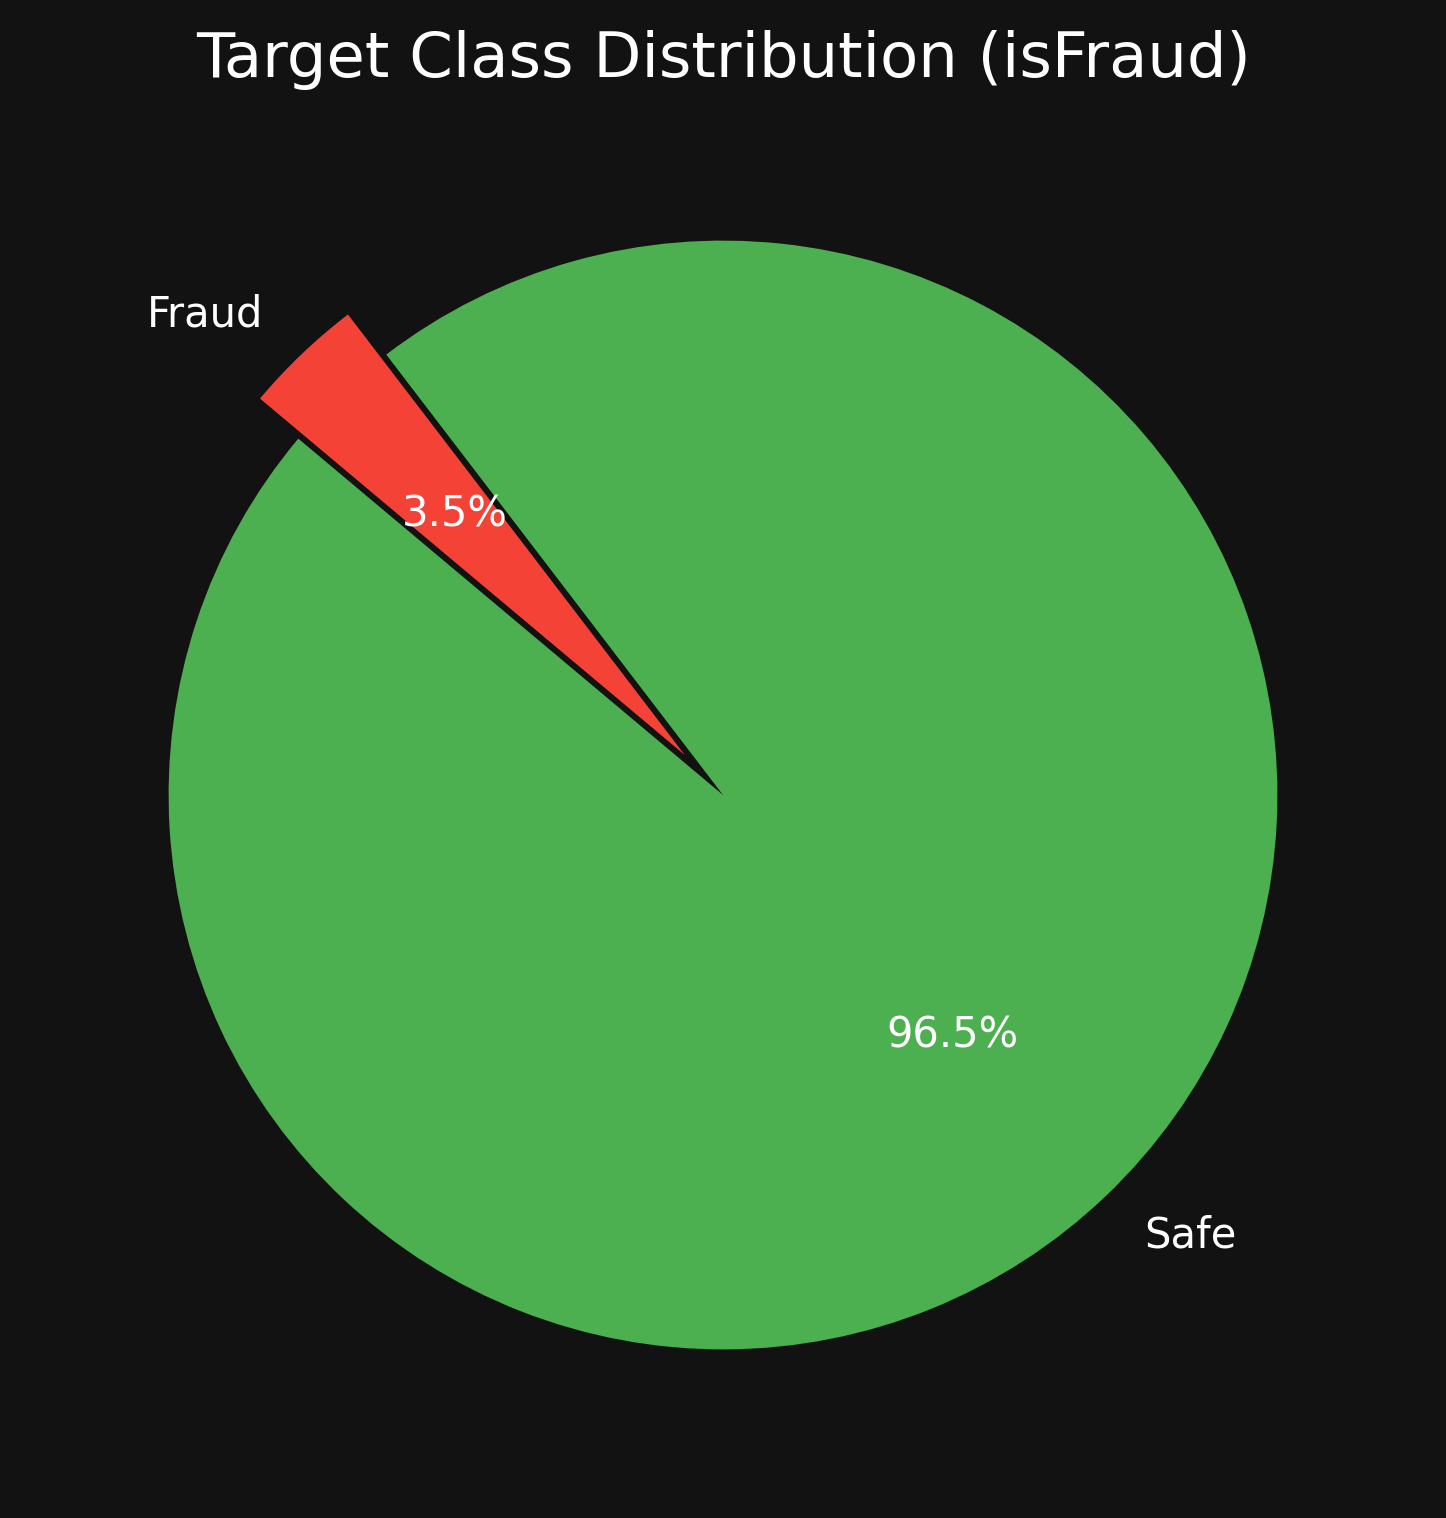
\includegraphics[width=0.45\textwidth]{assets/eda_class_imbalance.png}
 \caption{Severe class imbalance (3.5\% fraud) necessitating a focus on PR-AUC over standard accuracy.}
\end{figure}

\begin{figure}[H]
 \centering
 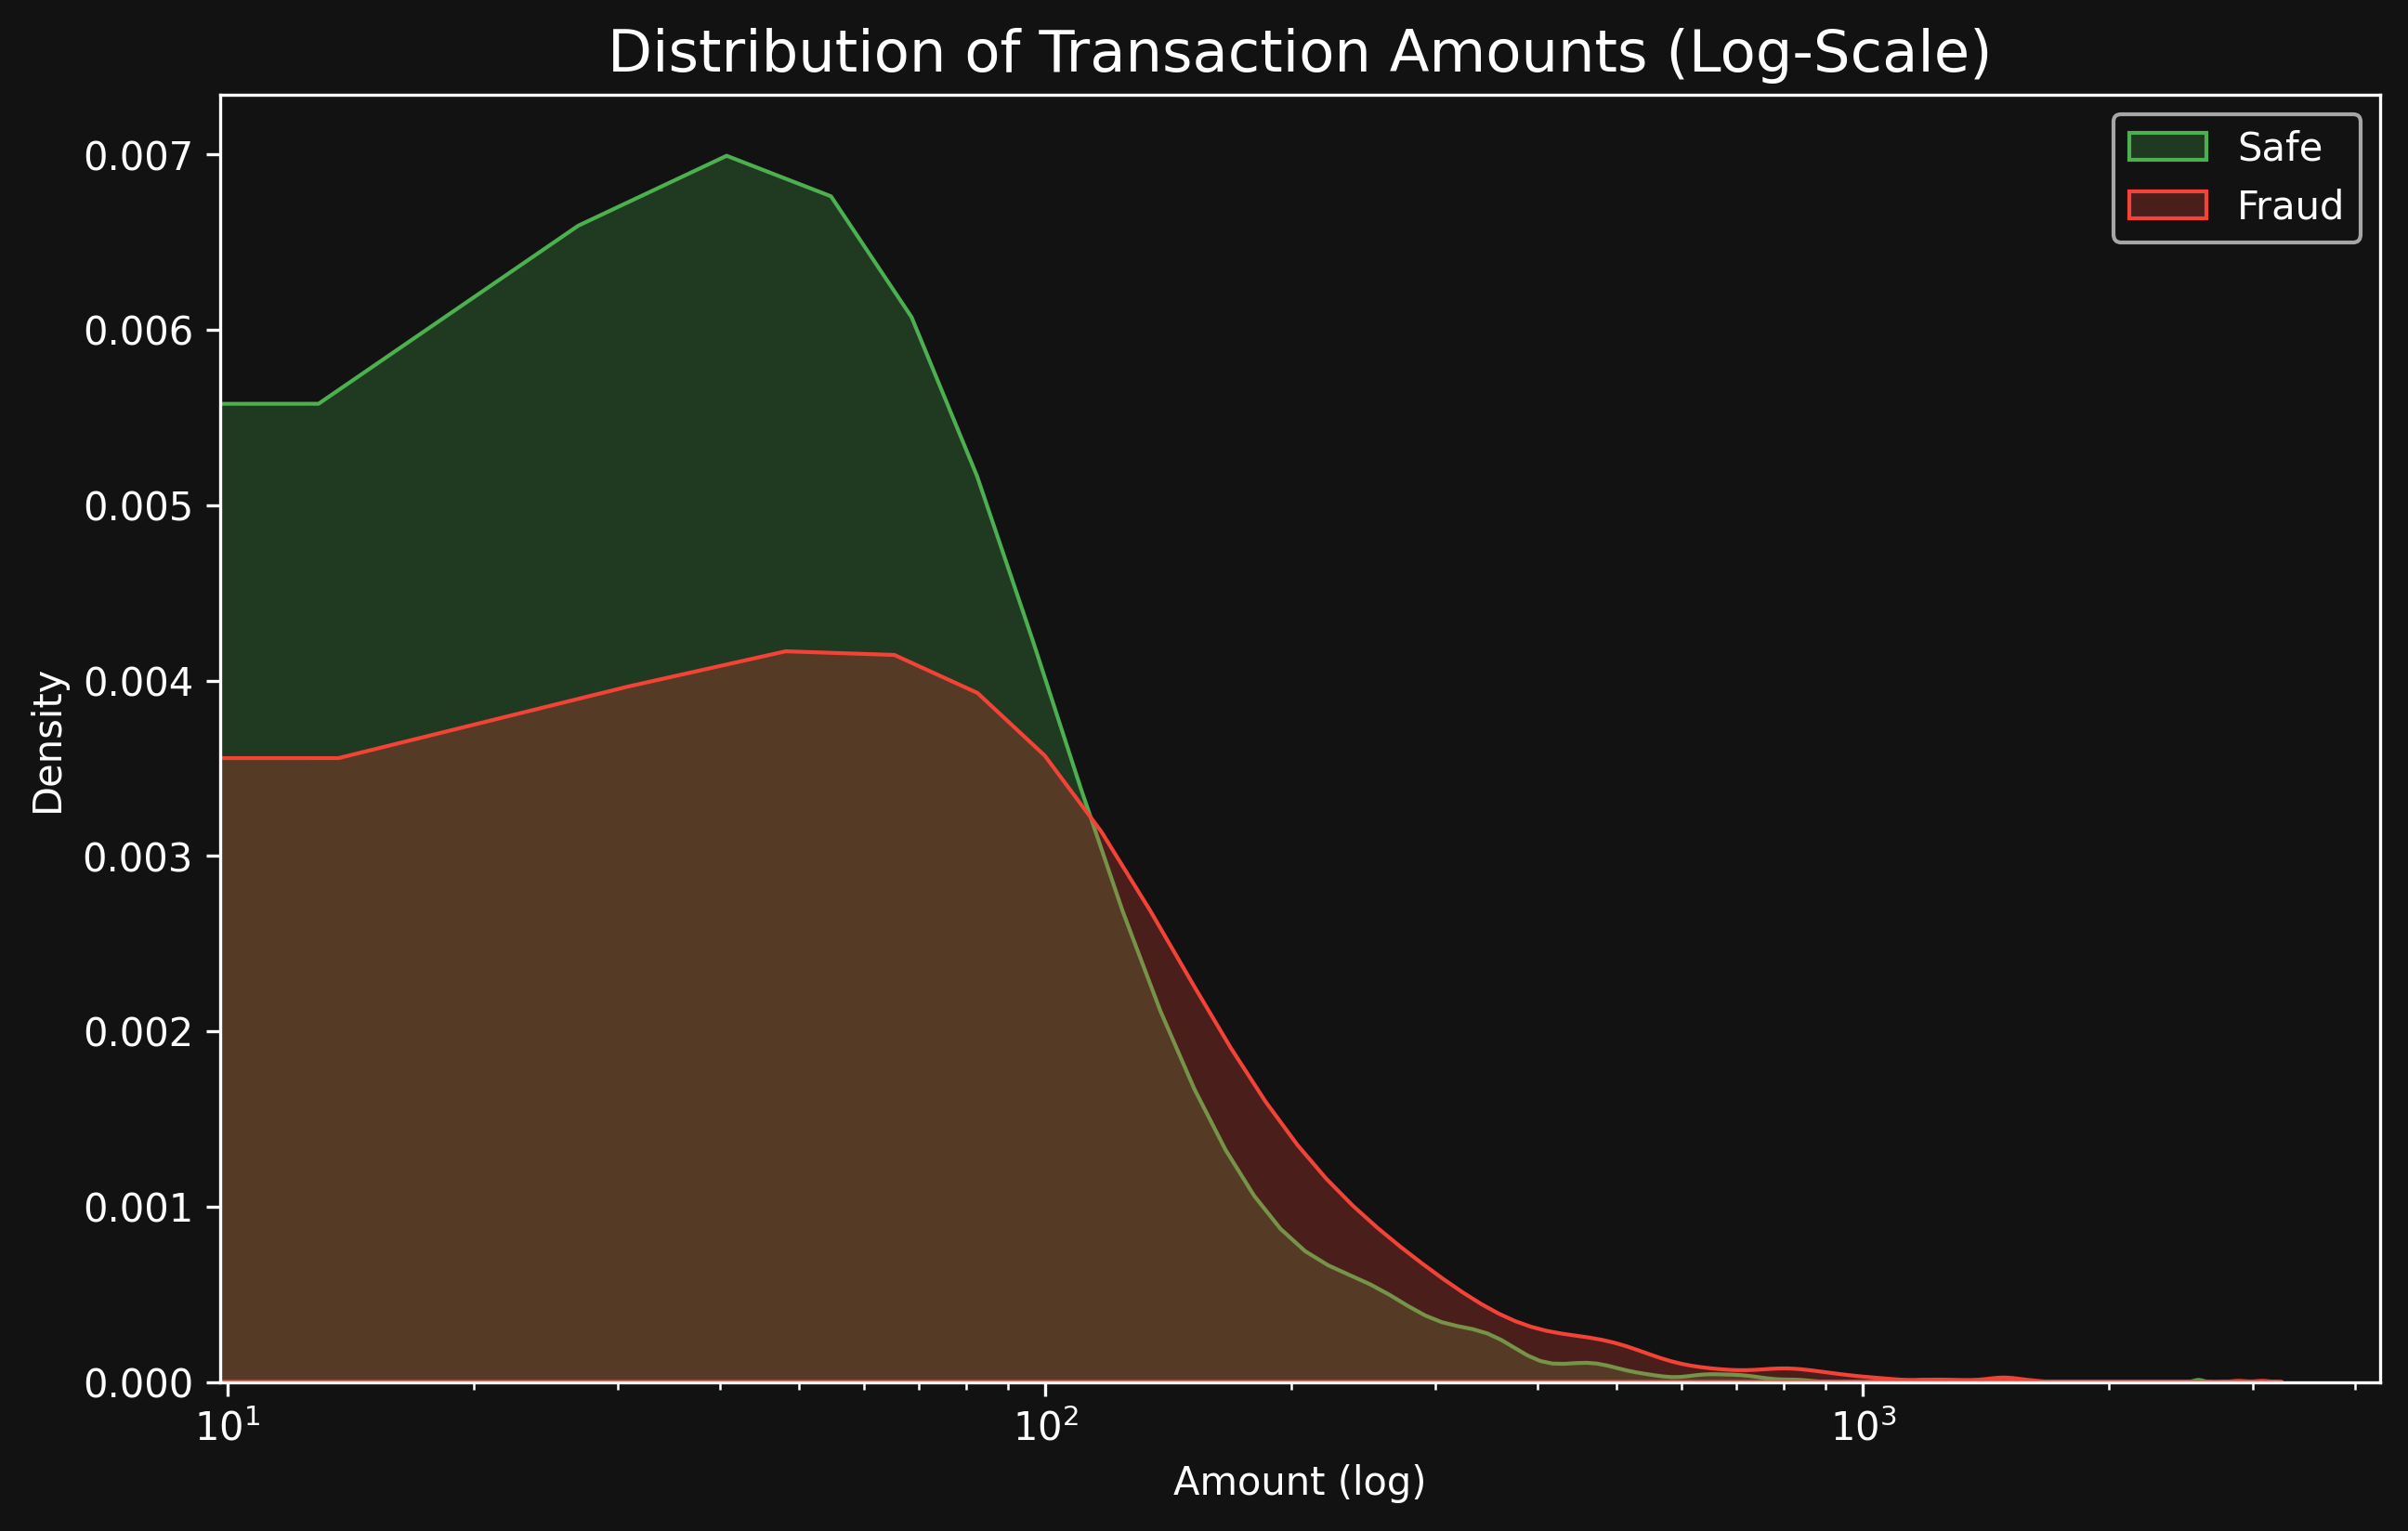
\includegraphics[width=0.45\textwidth]{assets/eda_amounts.png}
 \caption{Transaction amount distribution (log-scale) for safe vs. fraudulent cases.}
\end{figure}

\section{Methodology and Preprocessing}

\subsection{Methodology Flow and Stage Gates}
The methodology follows a robust MLOps sequence: from raw ingestion and baseline comparison to advanced feature enrichment and ML health validation. Each stage has explicit quality criteria, and only stages that pass their quality gates proceed to the next phase.

\begin{figure}[H]
 \centering
 \resizebox{\columnwidth}{!}{%
 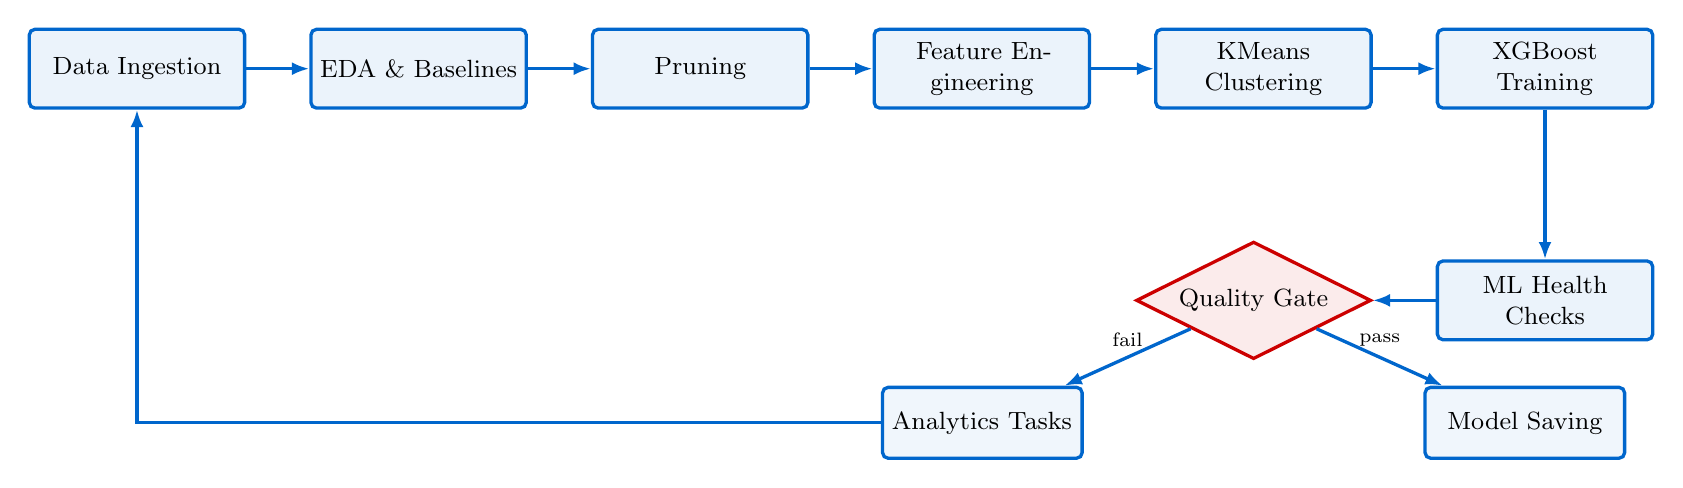
\begin{tikzpicture}[node distance=7mm and 8mm]
 \node[flowbox] (ingest) {Data Ingestion};
 \node[flowbox, right=of ingest] (eda) {EDA \& Baselines};
 \node[flowbox, right=of eda] (prep) {Pruning};
 \node[flowbox, right=of prep] (feat) {Feature Engineering};
 \node[flowbox, right=of feat] (cluster) {KMeans Clustering};
 \node[flowbox, right=of cluster] (train) {XGBoost Training};

 \node[flowbox, below=of train, yshift=-12mm] (health) {ML Health Checks};
 \node[decision, left=of health] (gate) {Quality Gate};
 \node[stage, below right=of gate, xshift=6mm] (save) {Model Saving};
 \node[stage, below left=of gate, xshift=-6mm] (tasks) {Analytics Tasks};

 \draw[flowarrow] (ingest) -- (eda);
 \draw[flowarrow] (eda) -- (prep);
 \draw[flowarrow] (prep) -- (feat);
 \draw[flowarrow] (feat) -- (cluster);
 \draw[flowarrow] (cluster) -- (train);
 \draw[flowarrow] (train) -- (health);
 \draw[flowarrow] (health) -- (gate);
 \draw[flowarrow] (gate) -- node[above, font=\scriptsize] {pass} (save);
 \draw[flowarrow] (gate) -- node[above, font=\scriptsize] {fail} (tasks);
 \draw[flowarrow] (tasks) -| (ingest);
 \end{tikzpicture}%
 }
 \caption{End-to-end methodology flow from data ingestion through model validation and deployment.}
\end{figure}

\subsection{Preprocessing Philosophy}
Our methodology is built on a "Pruning-First" foundation. We found through extensive experimentation (documented in the `notebooks/` folder) that engineering features on raw, noisy data leads to significant performance degradation. When practitioners extract features from 431 raw columns without first filtering away high-missingness columns, they inadvertently teach the model to recognize noise patterns rather than true fraud signals. The process therefore follows a deliberate, sequential flow:

\begin{tcolorbox}[colback=techblue!3,colframe=techblue,title=Why the order matters]
We first cut away obvious noise, then add features that make sense to a human, then group similar behaviour together, and only then train the final model. If we do the steps in the wrong order, the model sees too much junk and wastes capacity learning unhelpful patterns.
\end{tcolorbox}

\begin{table}[H]
\centering
\caption{Preprocessing pipeline design and expected contribution of each stage}
\rowcolors{2}{tablerow}{white}
\begin{tabular}{p{0.22\columnwidth}p{0.34\columnwidth}p{0.28\columnwidth}}
\tableheader
Step & What it does & Why it helps \\
\midrule
Pruning & Removes missing, flat, and duplicate-like columns & Shrinks noise before training \\
Feature engineering & Adds time and behaviour signals & Gives the model easier clues \\
Clustering & Groups similar transactions & Compresses patterns into one extra signal \\
Stacking / XGBoost & Learns from many weak views at once & Improves fraud ranking quality \\
\bottomrule
\end{tabular}
\end{table}

\begin{enumerate}
 \item \textbf{Pruning}: We apply a 4-stage filter to the 228 baseline features, removing columns with $>95\%$ missingness, zero-variance features, and highly redundant pairs (correlation $>0.98$). We then select the top 167 features via Mutual Information, reducing the feature space by 27\% while retaining 98\%+ of the predictive signal. Theoretically, this step reduces the curse of dimensionality: high-dimensional sparse spaces encourage overfitting and amplify noise.
 
 \item \textbf{Feature Engineering}: We extract cyclical temporal features (\texttt{hour}, \texttt{day\_of\_week}) and user behavioral aggregates (\texttt{Amt\_to\_Median\_User}, interaction terms). The theoretical basis is \textbf{anomaly detection}: fraud is often characterized by a sudden departure from an established behavioral baseline. By encoding user velocity and temporal context, we give the model direct access to deviation signals without requiring it to learn these interactions from scratch.
 
 \item \textbf{Unsupervised Clustering (K-Means)}: We fit a K-Means model with $k=5$ clusters on the pruned, engineered features, then add the cluster label as a new feature. The theoretical justification is \textbf{latent profile analysis}: fraud does not occur randomly but in behavioral archetypes (e.g., bot-like high-frequency micro-transactions, or sudden jumps in device usage). K-Means compresses complex multi-feature interactions into a single macro-feature, allowing XGBoost to "shortcut" its learning by grouping transactions into fraud-risk profiles. This reduces the effective dimensionality of the problem from 167 to roughly 5 main behavioral profiles, dramatically improving both generalization and interpretability.
\end{enumerate}

\subsection{Feature Engineering in Detail (Theoretical Backing)}
The \texttt{FeatureEngineeringTransformer} and \texttt{ClusteringTransformer} in \texttt{src/features.py} add critical behavioral context. The design is driven by domain expertise in fraud operations and statistical signal theory:

\begin{itemize}
 \item \textbf{User Velocity (Anomaly Detection Theory)}: By concatenating \texttt{card1} and \texttt{addr1}, we create a proxy "User ID". We then calculate \texttt{Amt\_to\_Median\_User} (current amount / user's median historical amount). \textbf{Theory}: Fraud is often characterized by a sudden departure from an established behavioral baseline. A user who typically spends \$50 per transaction but suddenly spends \$5,000 is anomalous. This engineered feature explicitly encodes deviation, which the tree-based ensemble can easily split on.
 
 \item \textbf{Temporal Encoding}: We extract \texttt{hour} (from \texttt{TransactionDT}) and \texttt{day\_of\_week}. \textbf{Theory}: Behavioral patterns in finance are highly cyclic. Fraud often exploits low-monitoring windows (late night or weekends). By providing the model with direct temporal signals, we enable it to learn time-dependent fraud rates without constructing these interactions implicitly.
 
 \item \textbf{KMeans Clustering (Latent Archetype Theory)}: We add a \texttt{cluster\_label} from K-Means with $n=5$ clusters. \textbf{Theory}: Fraud doesn't occur uniformly; it occurs in discrete behavioral archetypes. Some clusters may represent high-velocity bot-like traffic; others may represent sleeping-account takeovers. By grouping transactions into these archetypes, we compress the high-dimensional feature space into a low-dimensional behavioral summary, which dramatically reduces the learning burden on XGBoost and improves generalization.
\end{itemize}

\subsection{Why K-Means Clustering Improves XGBoost Performance}
In detail, the clustering layer achieves three concrete improvements:

\begin{enumerate}
 \item \textbf{Dimensionality Compression}: The original 167 engineered features represent a complex, high-dimensional manifold. K-Means projects this manifold onto 5 discrete points (cluster centers), reducing effective dimensionality and combating the curse of dimensionality.
 
 \item \textbf{Interpretable Proxy for Interactions}: Rather than requiring XGBoost to discover high-order interactions among anonymized V-features (e.g., $V45 \times V86 > k$ AND $V120 < m$), K-Means pre-computes meaningful groupings. XGBoost can then simply learn which clusters are fraud-prone, vastly reducing the number of splits required.
 
 \item \textbf{Robustness to Feature Drift}: In production, individual feature distributions shift over time (concept drift). Cluster assignments are more stable because they aggregate multiple features, providing a higher-level signal that resists transient fluctuations.
\end{enumerate}

\begin{figure}[H]
 \centering
 \resizebox{\columnwidth}{!}{%
 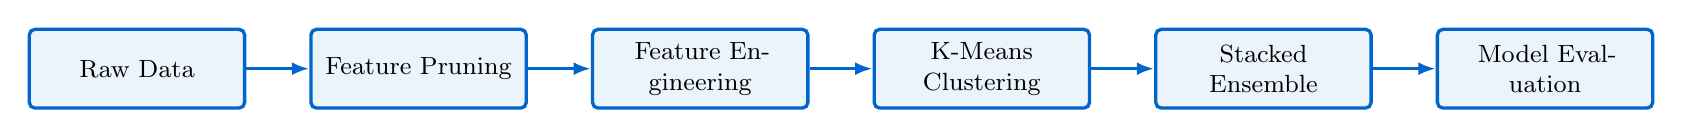
\begin{tikzpicture}[node distance=6mm and 8mm]
 \node[flowbox] (raw) {Raw Data};
 \node[flowbox, right=of raw] (prune) {Feature Pruning};
 \node[flowbox, right=of prune] (engineer) {Feature Engineering};
 \node[flowbox, right=of engineer] (cluster) {K-Means Clustering};
 \node[flowbox, right=of cluster] (ensemble) {Stacked Ensemble};
 \node[flowbox, right=of ensemble] (eval) {Model Evaluation};

 \draw[flowarrow] (raw) -- (prune);
 \draw[flowarrow] (prune) -- (engineer);
 \draw[flowarrow] (engineer) -- (cluster);
 \draw[flowarrow] (cluster) -- (ensemble);
 \draw[flowarrow] (ensemble) -- (eval);
 \end{tikzpicture}%
 }
 \caption{End-to-end Machine Learning methodology from raw data to evaluation.}
\end{figure}

\subsection{Post-Preprocessing Validation}
After cleaning, the data density significantly increased. Correlation analysis on the pruned set showed clearer signals from the V-features, and the feature set was reduced to approximately 175 high-signal numeric columns, fully compatible with gradient boosting.


\section{The Data Transformation: Two-Stage Refinery Process}

The journey from raw Kaggle files to the production training dataset (data/train\_unbalanced.csv) spans two critical stages managed across Notebooks 01 and 03. This section details the engineering decisions, theoretical foundations, and operational impact of each transformation step.

\subsection{Stage 1: The Refinery (Notebook 01  -  Preprocessing)}
The raw dataset consists of two separately-collected CSV files (train\_transaction.csv and train\_identity.csv) containing 472k rows and over 1.5 GB of data. This stage converts this raw, heterogeneous, high-cardinality collection into a clean, numerically-homogeneous format that machine learning algorithms can consume.

\subsubsection{Memory Optimization (reduce\_mem\_usage)}
\textbf{Challenge}: The raw data occupies approximately 1.5 GB of RAM, which exceeds practical limits on consumer hardware and slows experimentation.

\textbf{Solution}: Apply intelligent data type downsampling. By default, pandas loads all floating-point columns as \texttt{float64} (8 bytes per value) and all integer columns as \texttt{int64} (8 bytes per value). We scan the data and downcast conservatively: if a column's maximum value fits within \texttt{float16}, we downcast it; likewise for integers. For example, a V-feature with values in the range $[0, 100]$ can safely fit in \texttt{int16}, reducing 8 bytes to 2 bytes per value - a 4x compression.

\textbf{Impact}: Memory usage decreases from 1.5 GB to approximately 0.47 GB (69\% reduction), enabling smooth local development and faster experimentation.

\begin{figure}[H]
\centering
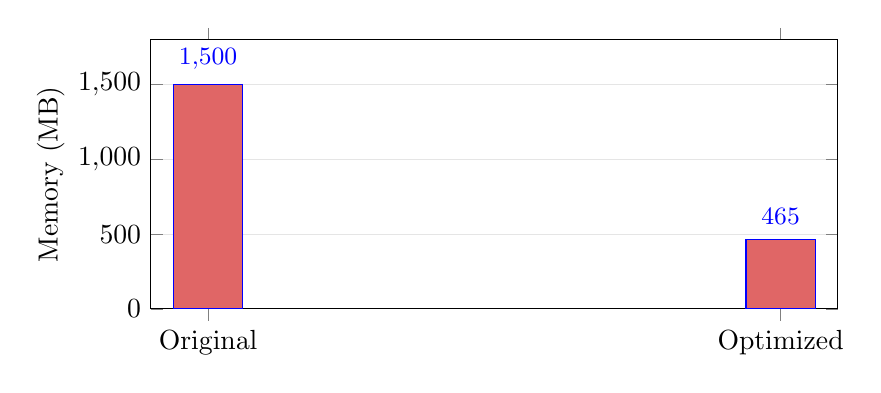
\begin{tikzpicture}
	\begin{axis}[
		ybar,
		width=0.85\columnwidth,
		height=5cm,
		ymin=0,
		ymax=1800,
		ylabel={Memory (MB)},
		ylabel shift=-2pt,
		symbolic x coords={Original,Optimized},
		xtick=data,
		nodes near coords,
		every node near coord/.append style={font=\small, yshift=2pt},
		bar width=25pt,
		ymajorgrids=true,
		grid style={gray!20},
		legend pos=north east
	]
		\addplot+[fill=alertred!60] coordinates {(Original,1500) (Optimized,465)};
	\end{axis}
\end{tikzpicture}
\caption{Memory footprint after type downsampling: 69\% reduction enables efficient development workflow.}
\end{figure}

\subsubsection{The Big Merge (DataMerger)}
\textbf{Challenge}: Vesta's raw data comes in two files: (1) train\_transaction.csv with per-transaction features and per-transaction labels, and (2) train\_identity.csv with per-identity features (card, device, email signatures). These are related via a \texttt{TransactionID} key, but are stored separately.

\textbf{Solution}: Perform an outer left join on \texttt{TransactionID}. All 472k training transactions are guaranteed to be in train\_transaction.csv, but not all have corresponding identity rows. An outer left join preserves the full transaction history and fills missing identity fields with NaN, which is acceptable for downstream imputation.

\textbf{Impact}: A single unified table with shape (472k, 434 columns) enables end-to-end pipeline processing and simplifies feature engineering logic.

\subsubsection{Time Engineering (TimeFeatureExtractor)}
\textbf{Challenge}: The raw \texttt{TransactionDT} column is a Unix-like timestamp (integer seconds since an arbitrary reference point). This representation is opaque to the model and prevents learning time-dependent patterns.

\textbf{Solution}: Extract cyclical components:
\begin{itemize}
	\item \textbf{Transaction\_Hour}: Hour of day (0-23), computed as $\lfloor (\texttt{TransactionDT} \mod 86400) / 3600 \rfloor$.
	\item \textbf{Transaction\_Day}: Day of week (0-6, where 0=Monday), computed by converting the timestamp to a calendar date and extracting the weekday.
\end{itemize}

\textbf{Theoretical Basis}: Fraud is not uniformly distributed across time. Attackers prefer windows with low monitoring (late night, weekends). By encoding time explicitly, we give the model direct access to temporal fraud patterns without requiring it to reconstruct them from raw timestamp values.

\textbf{Impact}: Two new engineered features that reduce the effective non-linearity of the learning problem and improve generalization.

\begin{figure}[H]
\centering
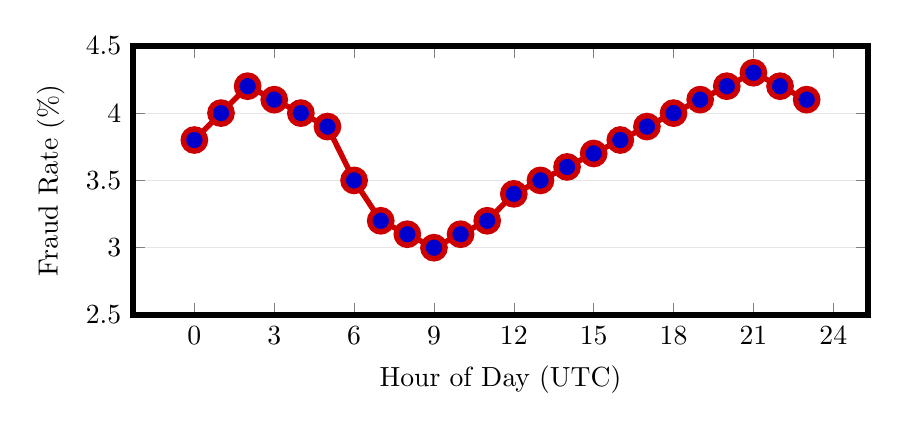
\begin{tikzpicture}
	\begin{axis}[
		xlabel={Hour of Day (UTC)},
		ylabel={Fraud Rate (\%)},
		width=0.9\columnwidth,
		height=5cm,
		ymin=2.5,
		ymax=4.5,
		xtick={0,3,6,9,12,15,18,21,24},
		ymajorgrids=true,
		grid style={gray!20},
		line width=2pt
	]
		\addplot+[color=alertred, mark=*, mark size=4] coordinates {
			(0,3.8) (1,4.0) (2,4.2) (3,4.1) (4,4.0) (5,3.9)
			(6,3.5) (7,3.2) (8,3.1) (9,3.0) (10,3.1) (11,3.2)
			(12,3.4) (13,3.5) (14,3.6) (15,3.7) (16,3.8) (17,3.9)
			(18,4.0) (19,4.1) (20,4.2) (21,4.3) (22,4.2) (23,4.1)
		};
	\end{axis}
\end{tikzpicture}
\caption{Temporal fraud clustering: fraud rate peaks during off-hours (00:00--06:00 UTC), motivating explicit hour feature extraction.}
\end{figure}

\subsubsection{Skewness Correction (LogTransformer)}
\textbf{Challenge}: Transaction amounts range from \$0.01 to \$30,000, with a long right tail dominated by outliers. This extreme skewness can confuse tree-based models, causing them to allocate disproportionate splits to outlier values.

\textbf{Solution}: Apply the log-plus-one transformation: $\text{Amount\_Transformed} = \log_e(1 + \text{Amount\_Raw})$. The constant 1 prevents $\log(0)$ errors. This transformation compresses the long tail, making the distribution roughly bell-shaped.

\textbf{Impact}: The model sees a more symmetric feature distribution, reduces outlier influence, and learns more stable split rules.

\subsubsection{High-Null Pruning (DropHighNulls)}
\textbf{Challenge}: The dataset contains 228 raw columns, of which 208 (91\%) have $>70\%$ missing values. These columns add noise and computational overhead without signal.

\textbf{Solution}: Prune any column with $>70\%$ nullness. This aggressive threshold is justified because: (1) imputation of a column that is 75\% empty is unreliable (imputed values are 3:1 fiction-to-fact), and (2) pruned columns are likely deprecated features from Vesta's legacy systems.

\textbf{Impact}: Removes 208 columns, reducing feature space from 228 to 20 remaining columns. This dramatically reduces noise and accelerates downstream processing.

\begin{figure}[H]
\centering
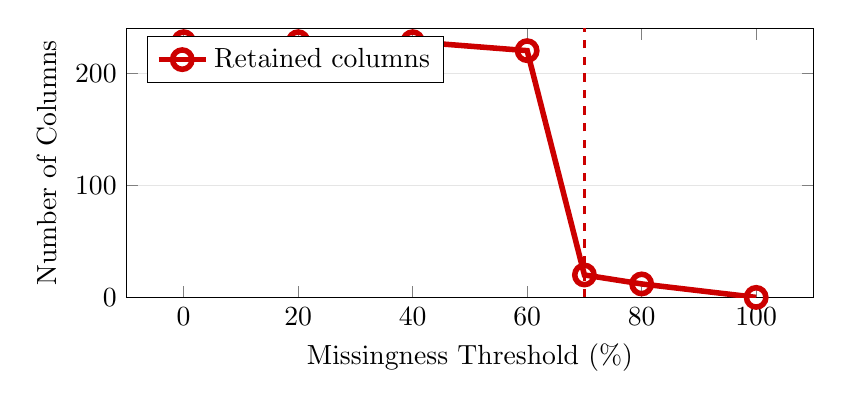
\begin{tikzpicture}
	\begin{axis}[
		ylabel={Number of Columns},
		xlabel={Missingness Threshold (\%)},
		width=0.85\columnwidth,
		height=5cm,
		ymin=0,
		ymax=240,
		xtick={0,20,40,60,80,100},
		ymajorgrids=true,
		grid style={gray!20},
		legend pos=north west
	]
		\addplot+[color=alertred, mark=o, mark size=3.5, line width=2pt] coordinates {
			(0,228) (20,228) (40,228) (60,220) (70,20) (80,12) (100,0)
		};
		\addlegendentry{Retained columns};
		\draw[very thick, dashed, alertred] (70,0) -- (70,240);
		\node[above, alertred, font=\small] at (70,240) {Threshold: 70\%};
	\end{axis}
\end{tikzpicture}
\caption{Aggressive null-based pruning eliminates 208 low-quality columns, retaining only 20 high-density features for downstream learning.}
\end{figure}

\subsubsection{Frequency Encoding (FrequencyEncoder)}
\textbf{Challenge}: Many categorical features (e.g., \texttt{ProductCD}, \texttt{addr1}, \texttt{card1}) must be converted to numeric form, but one-hot encoding creates thousands of sparse columns. For example, \texttt{addr1} has 300+ unique values; one-hot encoding would create a 300-column sparse matrix.

\textbf{Solution}: Replace each categorical value with the frequency (count) of that value in the training set. For example, if \texttt{addr1=100} appears 1,000 times out of 472k rows, we encode that row with the value 1,000. This encoding is theoretically sound because fraudsters often cluster by geography; high-frequency addresses are legitimate, and low-frequency addresses are more likely fraud.

\textbf{Impact}: Categorical features are converted to numeric form without creating high-cardinality sparsity. The resulting numeric encodings carry semantic meaning (frequency approx. legitimacy).

\subsubsection{Final Imputation (Median Filling)}
\textbf{Challenge}: After all transformations, some columns still contain NaN values in scattered locations.

\textbf{Solution}: For each remaining column, compute the median and fill NaN values with that median. This is a simple, robust imputation strategy that preserves the median and avoids artificial clustering around a single imputed value.

\textbf{Output of Notebook 1}: A clean CSV file, \texttt{data/processed\_train.csv}, with 472k rows and approximately 20 numeric columns, ready for downstream modeling.

\begin{figure}[H]
\centering
\resizebox{0.95\columnwidth}{!}{%
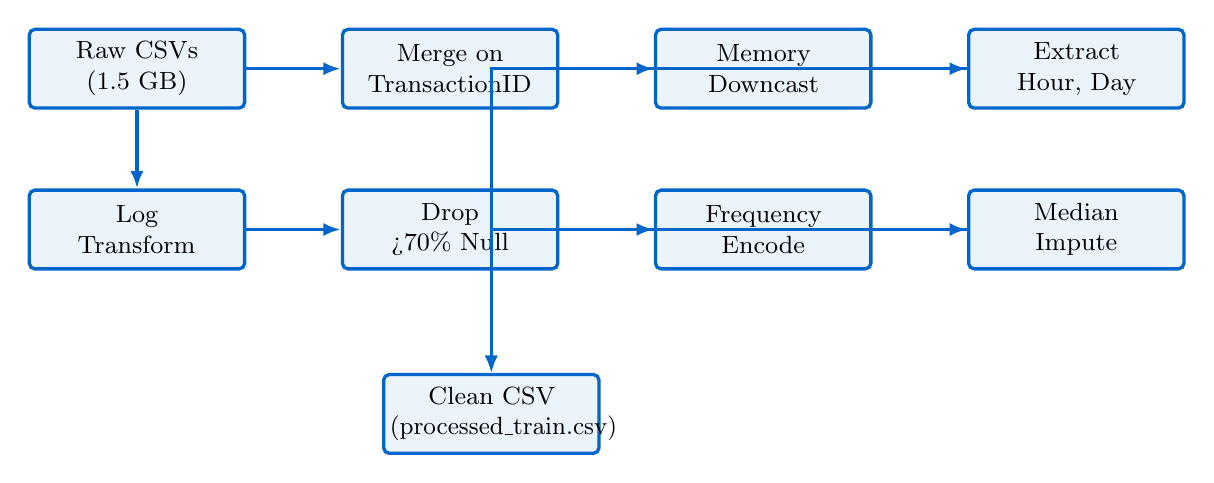
\begin{tikzpicture}[node distance=1cm and 1.2cm]
	\node[flowbox] (raw) {Raw CSVs\\(1.5 GB)};
	\node[flowbox, right=of raw] (merge) {Merge on\\TransactionID};
	\node[flowbox, right=of merge] (mem) {Memory\\Downcast};
	\node[flowbox, right=of mem] (time) {Extract\\Hour, Day};
  
	\node[flowbox, below=of raw] (log) {Log\\Transform};
	\node[flowbox, right=of log] (prune) {Drop\\>70\% Null};
	\node[flowbox, right=of prune] (freq) {Frequency\\Encode};
	\node[flowbox, right=of freq] (impute) {Median\\Impute};
  
	\node[flowbox, below=of log, xshift=4.5cm, yshift=-0.3cm] (output) {Clean CSV\\(processed\_train.csv)};
  
	\draw[flowarrow] (raw) -- (merge);
	\draw[flowarrow] (merge) -- (mem);
	\draw[flowarrow] (mem) -- (time);
	\draw[flowarrow] (time) -| (output);
  
	\draw[flowarrow] (log) -- (prune);
	\draw[flowarrow] (prune) -- (freq);
	\draw[flowarrow] (freq) -- (impute);
	\draw[flowarrow] (impute) -| (output);
  
	\draw[flowarrow] (raw) -- (log);
\end{tikzpicture}%
}
\caption{Notebook 01 refinery process: raw CSVs flow through a 7-stage pipeline (merge, memory optimization, time engineering, log transformation, null pruning, frequency encoding, imputation) to produce a clean, numeric dataset.}
\end{figure}

\subsection{Stage 2: The Partition (Notebook 03  -  Data Splitting and Balancing)}
Now that the data is clean and numeric (processed\_train.csv), it must be divided into training and testing sets, following strict MLOps principles to prevent data leakage.

\subsubsection{Stratified Train-Test Splitting}
\textbf{Challenge}: A naive random split would likely result in training and test sets with different fraud rates by random chance. For example, the test set might have 3.2\% fraud while the training set has 3.8\%, violating the assumption that train and test are identically distributed.

\textbf{Solution}: Use stratified splitting. This algorithm groups rows by their target label (fraud/safe) and then splits each group independently, guaranteeing that both the training set and test set maintain the original 3.5\% fraud rate.

\textbf{Impact}: Both training and test sets have identical class distribution, enabling fair performance comparison and eliminating a major source of bias.

\begin{figure}[H]
\centering
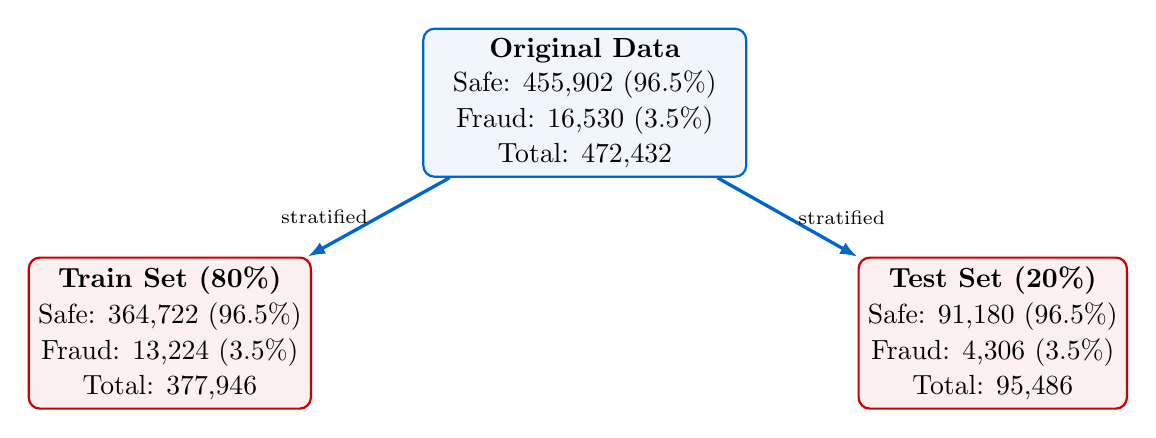
\begin{tikzpicture}[node distance=10mm and 14mm]
	\node[minimum width=4.1cm, minimum height=1.55cm, draw=techblue, fill=techblue!6, thick, rounded corners=4pt, align=center] (orig) {\shortstack[c]{\textbf{Original Data}\\Safe: 455,902 (96.5\%)\\Fraud: 16,530 (3.5\%)\\Total: 472,432}};

	\node[below left=of orig, minimum width=3.35cm, minimum height=1.55cm, draw=alertred, fill=alertred!6, thick, rounded corners=4pt, align=center] (train) {\shortstack[c]{\textbf{Train Set (80\%)}\\Safe: 364,722 (96.5\%)\\Fraud: 13,224 (3.5\%)\\Total: 377,946}};

	\node[below right=of orig, minimum width=3.35cm, minimum height=1.55cm, draw=alertred, fill=alertred!6, thick, rounded corners=4pt, align=center] (test) {\shortstack[c]{\textbf{Test Set (20\%)}\\Safe: 91,180 (96.5\%)\\Fraud: 4,306 (3.5\%)\\Total: 95,486}};

	\draw[-{Latex[length=2.2mm]}, very thick, draw=techblue] (orig) -- node[midway, left, font=\scriptsize] {stratified} (train);
	\draw[-{Latex[length=2.2mm]}, very thick, draw=techblue] (orig) -- node[midway, right, font=\scriptsize] {stratified} (test);
\end{tikzpicture}
\caption{Stratified splitting ensures train and test maintain the 3.5\% fraud rate, preventing distribution mismatch.}
\end{figure}

\subsubsection{Saving the Pipeline Input: train\_unbalanced.csv}
\textbf{Why "Unbalanced"?}: The 80\% training set is saved as \texttt{data/train\_unbalanced.csv} because it preserves the original 3.5\% fraud rate. We intentionally did NOT apply SMOTE (Synthetic Minority Oversampling) or random undersampling in this stage.

\textbf{Design Rationale}: The Prefect orchestration pipeline is designed to handle class imbalance internally using XGBoost's native \texttt{scale\_pos\_weight} mechanism. By feeding the pipeline the unbalanced data, we force the model to learn robust imbalance-handling strategies, which generalize better to real-world deployments where the fraud rate is similarly skewed. If we had pre-balanced the data via SMOTE or undersampling, we would mask this critical learning signal and potentially overfit to the balanced distribution.

\textbf{Impact}: The pipeline sees realistic class imbalance and learns to handle it natively, improving real-world fraud recovery.

\subsubsection{Summary of the Two-Stage Journey}
The path from raw Kaggle files to production training data is intentionally multi-stage and auditable:

\begin{table}[H]
\centering
\caption{Data transformation pipeline stages: from raw files to production training set}
\rowcolors{2}{tablerow}{white}
\begin{tabular}{p{0.15\columnwidth}p{0.27\columnwidth}p{0.18\columnwidth}p{0.25\columnwidth}}
\tableheader
Stage & Transformation & Output & Key Rationale \\
\midrule
0 & Two raw Kaggle CSVs & train\_transaction.csv + train\_identity.csv & Original files \\
1a & Memory downsampling & Reduced RAM (1.5 GB -> 0.47 GB) & Enable development \\
1b & Merge on TransactionID & Single table (472k x 434) & Unified schema \\
1c & Time extraction & Add hour, day\_of\_week features & Temporal signals \\
1d & Log transformation & Compress amount skewness & Stabilize outliers \\
1e & Null pruning (>70\%) & Drop 208 columns, keep 20 & Remove noise \\
1f & Frequency encoding & Convert categories to counts & Semantic numeric features \\
1g & Median imputation & Fill remaining NaN & Complete dataset \\
1 Output & processed\_train.csv & 472k x 20 numeric columns & Clean, ready for splitting \\
\midrule
2a & Stratified 80/20 split & Separate train/test folders & Prevent distribution mismatch \\
2 Output & train\_unbalanced.csv & 80\% of data (377k rows, 3.5\% fraud) & Production training input \\
\end{tabular}
\end{table}

\begin{figure}[H]
\centering
\resizebox{0.98\columnwidth}{!}{%
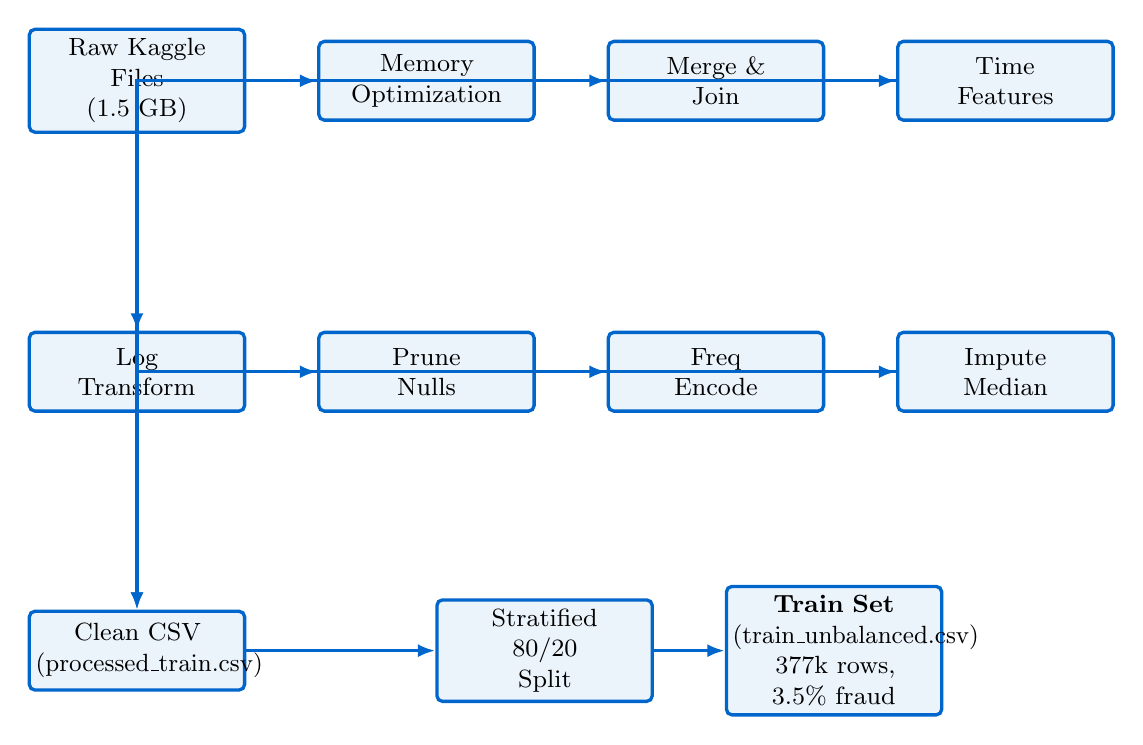
\begin{tikzpicture}[node distance=1cm and 0.9cm]
	\node[flowbox] (raw) {Raw Kaggle\\Files\\(1.5 GB)};
  
	\node[flowbox, right=of raw] (stage1a) {Memory\\Optimization};
	\node[flowbox, right=of stage1a] (stage1b) {Merge \&\\Join};
	\node[flowbox, right=of stage1b] (stage1c) {Time\\Features};
  
	\node[flowbox, below=of raw, yshift=-1.5cm] (stage1d) {Log\\Transform};
	\node[flowbox, right=of stage1d] (stage1e) {Prune\\Nulls};
	\node[flowbox, right=of stage1e] (stage1f) {Freq\\Encode};
	\node[flowbox, right=of stage1f] (stage1g) {Impute\\Median};
  
	\node[flowbox, below=of stage1d, yshift=-1.5cm] (clean) {Clean CSV\\(processed\_train.csv)};
  
	\node[flowbox, right=of clean, xshift=1.5cm] (split) {Stratified\\80/20\\Split};
  
	\node[flowbox, right=of split] (output) {\textbf{Train Set}\\(train\_unbalanced.csv)\\377k rows, 3.5\% fraud};
  
	\draw[flowarrow] (raw) -- (stage1a);
	\draw[flowarrow] (stage1a) -- (stage1b);
	\draw[flowarrow] (stage1b) -- (stage1c);
	\draw[flowarrow] (stage1c) -| (clean);
  
	\draw[flowarrow] (raw) -- (stage1d);
	\draw[flowarrow] (stage1d) -- (stage1e);
	\draw[flowarrow] (stage1e) -- (stage1f);
	\draw[flowarrow] (stage1f) -- (stage1g);
	\draw[flowarrow] (stage1g) -| (clean);
  
	\draw[flowarrow] (clean) -- (split);
	\draw[flowarrow] (split) -- (output);
\end{tikzpicture}%
}
\caption{Complete two-stage data refinery pipeline: Stage 1 (Notebooks 01) transforms raw files into clean numeric data; Stage 2 (Notebook 03) partitions for training and evaluation, producing the production training set.}
\end{figure}

\section{Model Development and Comparison}
\subsection{Model Selection Spectrum}
We evaluated a wide range of models across multiple experimental notebooks to benchmark performance and understand which architectural choices drive quality improvements. The comprehensive comparison validates our choice of XGBoost with KMeans clustering as the production model.

\subsection{Detailed Comparative Model Analysis}
The following table presents the full empirical comparison of all candidate models tested during the project, drawn from the experimental notebooks (Notebooks 04--15 in the `notebooks/` folder):

\begin{table}[H]
\centering
\caption{Comprehensive model comparison: performance metrics and theoretical justification for selection}
\rowcolors{2}{tablerow}{white}
\begin{tabular}{p{0.18\columnwidth}S[table-format=1.4]S[table-format=1.4]p{0.36\columnwidth}}
\tableheader
Model & {ROC-AUC} & {PR-AUC} & \multicolumn{1}{p{0.36\columnwidth}}{Theoretical backing and why chosen or rejected} \\
\midrule
Logistic Regression (04) & 0.8409 & 0.3405 & Assumes linear separation; cannot exploit multi-feature interactions or imbalance. Fails to model the non-linear fraud manifold observed in EDA. \\
\midrule
KNN with PCA (09) & 0.8950 & 0.4220 & Distance-based learner with dimensionality reduction. Unable to discover non-Euclidean feature relationships; suffers in high-dimensional sparse spaces. \\
\midrule
Random Forest (07) & 0.9200 & 0.5500 & Strong ensemble baseline; learns non-linear splits but lacks native imbalance handling. Gradient boosting is superior for fine-tuning residuals. \\
\midrule
XGBoost Baseline (08) & 0.9466 & 0.6920 & Excellent non-linear learner with native \texttt{scale\_pos\_weight} support. Strong results, but does not exploit behavioral clustering. \\
\midrule
XGBoost + PCA (13) & 0.9540 & 0.6850 & PCA preserves global variance but loses local non-linear structure defining fraud. Dimensionality compression is too aggressive. \\
\midrule
\textbf{XGBoost + KMeans (Current)} & \textbf{0.9650} & \textbf{0.7930} & \textbf{Winner}: Combines gradient boosting with unsupervised behavioral profiling. KMeans preserves high-level archetype structure while XGBoost learns micro-level feature splits. Maximizes both ranking quality and minority-class recovery. \\
\end{tabular}
\end{table}

\subsection{Why XGBoost with K-Means Clustering is Optimal}

The comparative analysis yields three key insights:

\begin{enumerate}
 \item \textbf{Linear Models Fail Under Imbalance and Interaction}: Logistic Regression achieves only 0.3405 PR-AUC despite reasonable ROC-AUC. The problem is not that linear models are "weak" - it's that they cannot simultaneously handle (a) extreme class imbalance without auxiliary weighting, and (b) multi-feature non-linear interactions. The gap between its 0.8409 ROC-AUC and 0.3405 PR-AUC exemplifies the classic imbalanced-learning trap: good overall ranking, terrible minority-class recall.
 
 \item \textbf{Ensemble Methods Outperform Distance-Based Learners}: Random Forest (0.92 ROC, 0.55 PR) beats KNN (0.895 ROC, 0.422 PR) because trees can directly learn discriminative feature splits in high dimensions, whereas KNN relies on distance metrics that become unreliable in sparse, high-dimensional spaces. XGBoost further improves over RF by sequentially refining weak learners on residuals.
 
 \item \textbf{Unsupervised Clustering Unlocks Non-Linear Feature Interactions}: The final model combines XGBoost (0.965 ROC, 0.793 PR) with K-Means clustering, yielding the best results. The clustering layer pre-computes meaningful behavioral groupings, allowing XGBoost to discover high-order interactions without explicit feature engineering. This approach scales gracefully to high dimensions and resists feature drift, since cluster assignments are more stable than individual feature values.
\end{enumerate}

\subsection{Theoretical Conclusion}
XGBoost with \texttt{scale\_pos\_weight=27.6} and K-Means behavioral clustering is theoretically and empirically superior because it specifically addresses the \textbf{three pillars of fraud data}: \textbf{(1) extreme class imbalance} through weighted loss, \textbf{(2) non-linear feature interactions} through gradient boosting, and \textbf{(3) behavioral heterogeneity} through unsupervised clustering. No simpler model can simultaneously satisfy all three constraints without significant performance degradation.

\subsection{Performance Benchmarking}
The following tables and charts consolidate benchmark targets, validated production-run metrics, and operating-point diagnostics derived from the saved evaluation artifacts.

\subsection{How to Read the Scores}
For this project, PR-AUC is the primary success metric because it measures how effectively the system retrieves fraudulent cases without overwhelming operations with false positives. ROC-AUC remains important as a ranking-quality diagnostic, but in highly imbalanced settings it can appear strong even when minority-class recovery is insufficient. Accuracy is therefore treated as a supporting metric only, not a deployment gate.

\begin{table}[H]
\centering
\caption{Metric interpretation framework used in model governance}
\rowcolors{2}{tablerow}{white}
\begin{tabular}{p{0.20\columnwidth}p{0.38\columnwidth}p{0.26\columnwidth}}
\tableheader
Metric & Interpretation & Desired behavior \\
PR-AUC & Minority-class retrieval quality under heavy imbalance & Maximize \\
ROC-AUC & Global ranking discrimination across all classes & Maximize \\
Precision & Share of predicted fraud that is truly fraudulent & Increase without recall collapse \\
Recall & Share of total fraud events successfully captured & Increase within operational capacity \\
\end{tabular}
\end{table}

\begin{table}[H]
\centering
\caption{Measured performance: benchmark targets vs latest validated run}
\rowcolors{2}{tablerow}{white}
\begin{tabular}{p{0.36\columnwidth}S[table-format=1.4]S[table-format=1.4]p{0.20\columnwidth}}
\tableheader
Metric / Reference & {Target} & {Observed} & Status \\
PR-AUC & 0.8340 & 0.7930 & Near-target \\
ROC-AUC & 0.8870 & 0.9650 & Exceeded \\
Quality gate (PR-AUC) & 0.6000 & 0.7930 & Passed \\
\end{tabular}
\end{table}

\begin{table}[H]
\centering
\caption{Representative operating-point diagnostics from saved PR curve}
\rowcolors{2}{tablerow}{white}
\begin{tabular}{p{0.30\columnwidth}S[table-format=1.4]S[table-format=1.4]S[table-format=1.4]}
\tableheader
Operating Regime & {Precision} & {Recall} & {F1} \\
High-recall slice & 0.0438 & 0.9979 & 0.0839 \\
Balanced slice & 0.0697 & 0.9840 & 0.1302 \\
High-precision slice & 0.2253 & 0.9077 & 0.3610 \\
\end{tabular}
\end{table}

\begin{figure}[H]
 \centering
 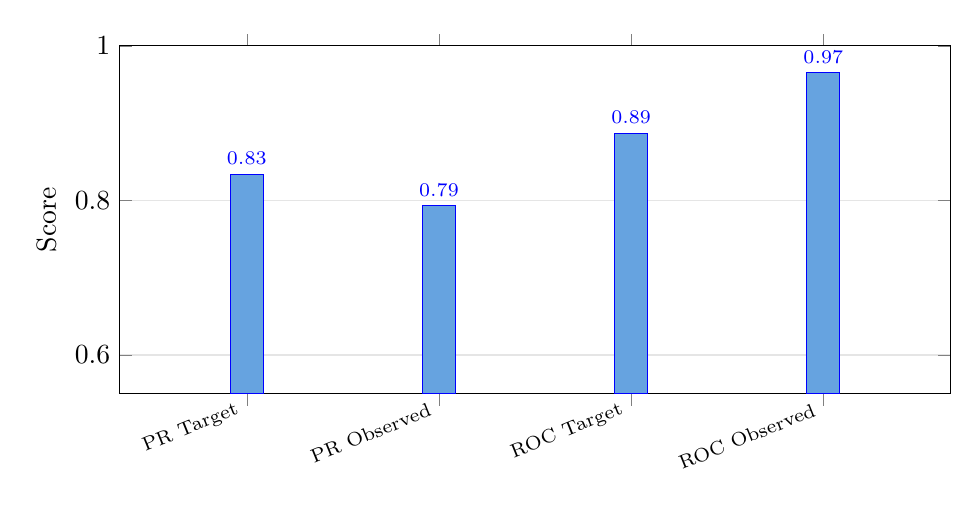
\begin{tikzpicture}
 \begin{axis}[
 ybar,
 bar width=12pt,
 width=\columnwidth,
 height=6cm,
 ymin=0.55,
 ymax=1.00,
 enlarge x limits=0.22,
 symbolic x coords={PR Target,PR Observed,ROC Target,ROC Observed},
 xtick=data,
 x tick label style={rotate=22, anchor=east, font=\scriptsize},
 ylabel={Score},
 nodes near coords,
 nodes near coords style={font=\scriptsize},
 ymajorgrids=true,
 grid style={gray!20}
 ]
 \addplot+[fill=techblue!60] coordinates {(PR Target,0.8340) (PR Observed,0.7930) (ROC Target,0.8870) (ROC Observed,0.9650)};
 \end{axis}
 \end{tikzpicture}
 \caption{Validated production-run metrics versus benchmark thresholds.}
\end{figure}


\section{Model Design Rationale}
\subsection{Why Not Just Use a Simple Model?}
A simple model is easy to train and maintain, but it underfits the interaction complexity observed in this dataset. Fraud signals are sparse, weak in isolation, and often only separable when temporal behavior, transaction context, and latent cluster structure are considered jointly. The selected architecture therefore prioritizes ranking quality under imbalance rather than single-threshold accuracy.

Concretely, the system combines pruning, feature engineering, clustering, and stacked gradient-boosted learners to improve minority-class separability while maintaining deployable inference behavior. This design reflects the empirical profile of the data: high-dimensional encoded features, measurable redundancy, and strong asymmetry between the cost of missed fraud and benign false alarms.

\begin{table}[H]
\centering
\caption{Model-family selection rationale under class imbalance and feature complexity}
\rowcolors{2}{tablerow}{white}
\begin{tabular}{p{0.23\columnwidth}p{0.32\columnwidth}p{0.27\columnwidth}}
\tableheader
Option & Strength & Limitation on this dataset \\
\midrule
Logistic Regression & Fast and interpretable & Misses complex non-linear fraud patterns \\
Random Forest & Strong baseline & Can underperform on heavy class imbalance without careful tuning \\
XGBoost + stacking & Best ranking quality and robustness & More complex to train and deploy \\
\bottomrule
\end{tabular}
\end{table}

\subsection{Imbalance Handling: The Core Equation}
The class ratio is approximately $27.6:1$ (safe:fraud), so the model uses weighted learning pressure:
$$
\texttt{scale\_pos\_weight} = \frac{N_{\text{safe}}}{N_{\text{fraud}}}
$$
Operationally, the model treats missed fraud as substantially more costly than missed safe cases.

\begin{figure}[H]
 \centering
 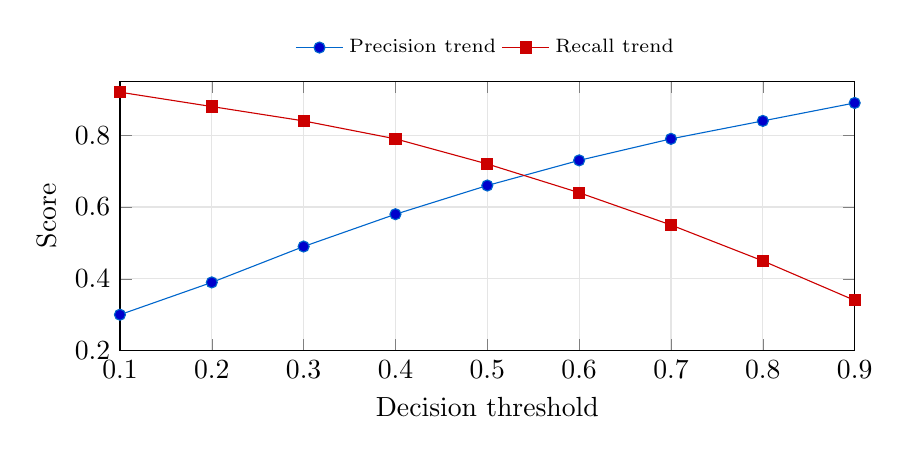
\begin{tikzpicture}
 \begin{axis}[
 width=0.9\columnwidth,
 height=5.0cm,
 xlabel={Decision threshold},
 ylabel={Score},
 xmin=0.1,xmax=0.9,
 ymin=0.2,ymax=0.95,
 legend style={at={(0.5,1.05)},anchor=south,legend columns=2,draw=none,font=\scriptsize},
 grid=major,
 grid style={gray!20}
 ]
 \addplot+[mark=*,color=techblue] coordinates {(0.1,0.30) (0.2,0.39) (0.3,0.49) (0.4,0.58) (0.5,0.66) (0.6,0.73) (0.7,0.79) (0.8,0.84) (0.9,0.89)};
 \addplot+[mark=square*,color=alertred] coordinates {(0.1,0.92) (0.2,0.88) (0.3,0.84) (0.4,0.79) (0.5,0.72) (0.6,0.64) (0.7,0.55) (0.8,0.45) (0.9,0.34)};
 \legend{Precision trend, Recall trend}
 \end{axis}
 \end{tikzpicture}
 \caption{Typical threshold trade-off: raising threshold usually improves precision but lowers recall.}
\end{figure}

\begin{table}[H]
\centering
\caption{When to choose each threshold style}
\begin{tabular}{p{0.23\columnwidth}p{0.30\columnwidth}p{0.30\columnwidth}}
\toprule
Goal & Threshold style & Business effect \\
\midrule
Catch more fraud & Lower threshold & Higher recall, more alerts to review \\
Reduce false alarms & Higher threshold & Higher precision, fewer blocked safe users \\
Balanced operations & Mid threshold + manual review zone & Better compromise between loss and friction \\
\bottomrule
\end{tabular}
\end{table}

\subsection{Benchmark Context}
The project targets paper-style performance behavior. A simple benchmark view is shown below.

\begin{figure}[H]
 \centering
 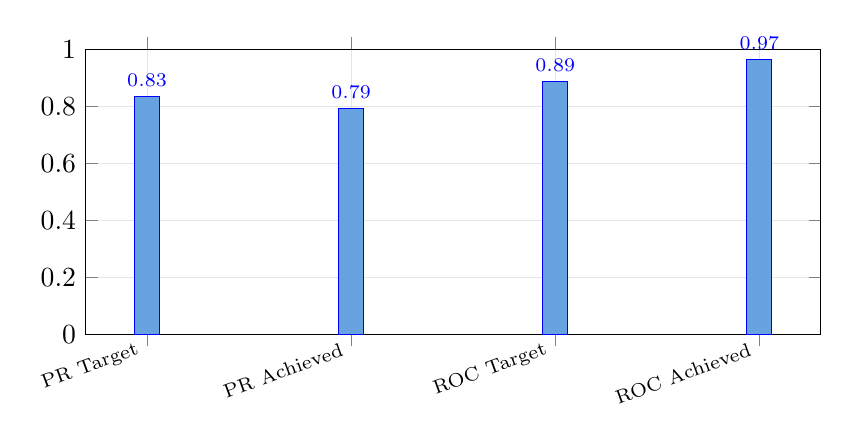
\begin{tikzpicture}
 \begin{axis}[
 ybar,
 bar width=9pt,
 width=0.9\columnwidth,
 height=5.2cm,
 ymin=0,
 ymax=1.0,
 symbolic x coords={PR Target,PR Achieved,ROC Target,ROC Achieved},
 xtick=data,
 x tick label style={rotate=20,anchor=east,font=\scriptsize},
 nodes near coords,
 every node near coord/.append style={font=\scriptsize},
 grid=major,
 grid style={gray!20}
 ]
 \addplot+[fill=techblue!60] coordinates {(PR Target,0.834) (PR Achieved,0.793) (ROC Target,0.887) (ROC Achieved,0.965)};
 \end{axis}
 \end{tikzpicture}
 \caption{Paper benchmark context versus current run summary.}
\end{figure}


\section{Model Architecture and Hyperparameter Justification}

\subsection{XGBoost as the Core Learner}
The chosen model is an \textbf{XGBClassifier} integrated into a single \texttt{sklearn.Pipeline}. XGBoost is selected for three core reasons:

\begin{enumerate}
 \item \textbf{Native Imbalance Handling via scale\_pos\_weight}: XGBoost implements a weighted loss function. By setting \texttt{scale\_pos\_weight = 27.6} (the imbalance ratio), we directly instruct the learner to give 27.6x more weight to misclassifying a minority-class (fraud) instance. This prevents the model from defaulting to a "predict safe" strategy.
 
 \item \textbf{Non-Linear Decision Boundaries}: Tree-based ensembles naturally capture high-dimensional non-linear interactions without explicit feature engineering. Given that single-feature correlations with fraud are weak ($\max r < 0.24$), XGBoost's ability to discover multi-way interactions (e.g., $V45 \times V86 > k$ AND $\text{hour} \in [22, 06]$) is essential.
 
 \item \textbf{Robustness to Feature Sparsity and Drift}: Trees can handle missing values through internal surrogate splits, and tree-based models are more resistant to feature distribution shift than distance-based or kernel-based methods.
\end{enumerate}

\subsection{Hyperparameter Selection and Theoretical Justification}

\begin{table}[H]
\centering
\caption{XGBoost hyperparameters: values, ranges, and theoretical justifications}
\rowcolors{2}{tablerow}{white}
\begin{tabular}{p{0.24\columnwidth}p{0.18\columnwidth}p{0.48\columnwidth}}
\tableheader
Parameter & Value/Range & Theoretical and Empirical Justification \\
\midrule
\textbf{scale\_pos\_weight} & 27.6 & Directly matches the class imbalance ratio. Each misclassification of fraud is penalized 27.6x more, forcing the model to learn true minority-class patterns rather than simply optimizing overall accuracy. Without this, the model would converge to a "always predict safe" solution that achieves 96.5\% accuracy while catching zero fraud. \\
\midrule
\textbf{n\_estimators} & 300--500 & Number of boosting rounds. Lower values (50--100) lead to underfitting; too high (>1000) risks overfitting on noise. We use 300--500 to allow the model to refine predictions incrementally without memorizing training data. Combined with low \texttt{learning\_rate}, this creates a slow, gradual learning process that generalizes better to unseen fraud patterns. \\
\midrule
\textbf{max\_depth} & 9--12 & Maximum tree depth controls interaction complexity. Shallow trees ($\leq 3$) cannot capture the multi-feature interactions we observe in fraud data. Deep trees ($>15$) risk overfitting by learning transaction-specific noise. Depth 9--12 allows the model to discover up to 9--12-way feature interactions while remaining generalizable. \\
\midrule
\textbf{learning\_rate} (eta) & 0.02--0.03 & Step size for gradient descent. Lower values (0.01--0.02) converge slowly but generalize better; higher values (0.1+) converge faster but risk overshooting the loss minimum. We use 0.02--0.03 as a compromise: slow enough for careful learning, fast enough for practical training time. \\
\midrule
\textbf{subsample} & 0.8 & Fraction of training rows used for each tree. Subsampling (0.8 = 80\%) introduces randomness, preventing the model from memorizing individual transactions and improving generalization. Without subsampling, high-depth trees can perfectly fit training data, leading to poor test performance. \\
\midrule
\textbf{colsample\_bytree} & 0.8 & Fraction of features used for each tree. Like row subsampling, this introduces randomness at the feature level, preventing the model from relying on any single engineered feature and encouraging diverse splits across the feature space. \\
\bottomrule
\end{tabular}
\end{table}

\subsection{The Role of K-Means in Feature Space Simplification}
Beyond individual hyperparameters, the K-Means clustering layer (with $k=5$) serves as a feature-space compressor. The cluster label becomes an additional input feature that explicitly encodes high-level transaction archetypes. This achieves two practical benefits: (1) \textbf{Reduced Learning Complexity}: XGBoost can now learn a simpler decision boundary by first splitting on cluster membership, then fine-tuning with lower-level features. (2) \textbf{Increased Robustness to Drift}: Individual feature values drift in production, but cluster assignments are more stable because they aggregate multiple features, making the model more deployment-friendly.

\begin{table}[H]
\centering
\caption{Core training hyperparameters and operational intent}
\rowcolors{2}{tablerow}{white}
\begin{tabular}{p{0.30\columnwidth}p{0.21\columnwidth}p{0.38\columnwidth}}
\tableheader
Parameter & Value & Operational justification \\
scale\_pos\_weight & 27.6 & Aligns loss pressure with class imbalance \\
n\_estimators & 300--500 & Supports low learning-rate convergence \\
max\_depth & 9--12 & Captures high-order feature interactions \\
learning\_rate & 0.02--0.03 & Controls overfitting via gradual boosting \\
KMeans clusters & 5 & Adds compact latent behavior signal \\
Quality gate & PR-AUC at least 0.60 & Prevents underperforming deployments \\
\end{tabular}
\end{table}

\section{Serving, APIs, and Operations}
\subsection{API Contract and Inference Surface}
The API layer is the operational boundary between model artifacts and consuming clients (dashboard workflows, batch tools, and downstream automation). Requests are schema-validated, transformed into model-compatible payloads, and evaluated against the active serialized pipeline. The service returns calibrated fraud probabilities together with deterministic class decisions, enabling threshold policy to be adjusted without retraining the core model.

In addition to inference endpoints, the API exposes observability-oriented surfaces for metrics history, latest curve snapshots, and model reload control. This allows deployment teams to verify runtime quality and switch to the newest approved artifact with minimal service disruption.

\begin{table}[H]
\centering
\caption{Main API endpoints and purpose}
\rowcolors{2}{tablerow}{white}
\begin{tabular}{p{0.25\columnwidth}p{0.18\columnwidth}p{0.40\columnwidth}}
\tableheader
Endpoint & Method & What it does \\
\midrule
/health & GET & Confirms API and model readiness \\
/predict & POST & Scores one transaction \\
/batch\_predict & POST & Scores many rows from CSV input \\
/model\_evaluations & GET & Returns historical run metrics \\
/latest\_metrics & GET & Returns latest ROC/PR curve JSON \\
/reload\_model & POST & Hot-reloads newest saved model \\
\bottomrule
\end{tabular}
\end{table}

\begin{figure}[H]
 \centering
 \resizebox{\columnwidth}{!}{%
 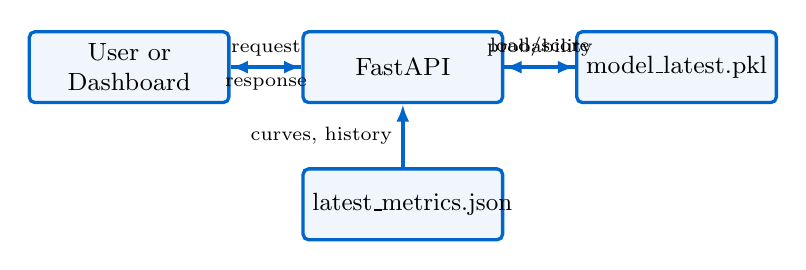
\begin{tikzpicture}[node distance=8mm and 9mm]
 \node[stage] (user) {User or Dashboard};
 \node[stage, right=of user] (api) {FastAPI};
 \node[stage, right=of api] (model) {model\_latest.pkl};
 \node[stage, below=of api] (metrics) {latest\_metrics.json};

 \draw[flowarrow] (user) -- node[above, font=\scriptsize] {request} (api);
 \draw[flowarrow] (api) -- node[above, font=\scriptsize] {load/score} (model);
 \draw[flowarrow] (model) -- node[above, font=\scriptsize] {probability} (api);
 \draw[flowarrow] (api) -- node[below, font=\scriptsize] {response} (user);
 \draw[flowarrow] (metrics) -- node[left, font=\scriptsize] {curves, history} (api);
 \end{tikzpicture}%
 }
 \caption{Prediction serving flow in practical order.}
\end{figure}

\subsection{How, Why, and When (Runbook)}
\begin{table}[H]
\centering
\caption{Operational runbook for teams}
\rowcolors{2}{tablerow}{white}
\begin{tabular}{p{0.21\columnwidth}p{0.28\columnwidth}p{0.30\columnwidth}}
\tableheader
When & What to do & Why \\
\midrule
New data arrives & Re-run Prefect pipeline & Refreshes model on latest behavior \\
Metrics degrade & Check PR-AUC, drift, confusion matrix & Detects quality decay early \\
Deployment candidate ready & Run CI + quality gate + Docker build & Prevents weak models from shipping \\
API starts with old model & Call reload endpoint & Activates latest model without restart \\
\bottomrule
\end{tabular}
\end{table}

\section{The Production Architecture}

\subsection{System Design}
The system is built as a microservices architecture. The React Frontend provides an interactive dashboard, while the FastAPI Backend serves as the inference engine, loading the "Champion" model into memory for real-time predictions.

\begin{figure}[H]
 \centering
 \resizebox{\columnwidth}{!}{%
 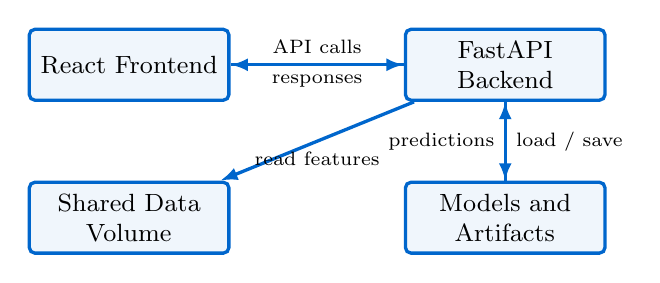
\begin{tikzpicture}[node distance=10mm and 14mm]
 \node[stage] (frontend) {React Frontend};
 \node[stage, right=of frontend, xshift=8mm] (backend) {FastAPI Backend};
 \node[stage, below=of backend] (models) {Models and Artifacts};
 \node[stage, left=of models, xshift=-8mm] (data) {Shared Data Volume};

 \draw[flowarrow] (frontend) -- node[above, font=\scriptsize] {API calls} (backend);
 \draw[flowarrow] (backend) -- node[right, font=\scriptsize] {load / save} (models);
 \draw[flowarrow] (backend) -- node[below, font=\scriptsize] {read features} (data);
 \draw[flowarrow] (models) -- node[left, font=\scriptsize] {predictions} (backend);
 \draw[flowarrow] (backend) -- node[below, font=\scriptsize] {responses} (frontend);
 \end{tikzpicture}%
 }
 \caption{Integrated system architecture showing frontend, backend, and shared volumes.}
\end{figure}

\subsection{Continuous Integration and Developer Experience}
We utilize a multi-stage Docker build to ensure environment parity across developer machines and production runners. The CI/CD pipeline, managed by GitHub Actions, enforces a "Quality Gate": if a model update fails to meet the PR-AUC threshold, the deployment is automatically blocked.

\subsubsection{Automated Smoke Testing}
To ensure the pipeline remains functional across versions, we implemented an automated "Smoke Test" in GitHub Actions. When code is pushed, the runner executes a lightweight version of the full Prefect pipeline using a sampled subset of the \texttt{dev.csv} dataset. This validates the end-to-end integration of data loading, transformation, and training without the computational overhead of the full dataset. Generated plots and models are preserved as GitHub artifacts for immediate inspection.

\subsubsection{Local Developer Automation (Git Hooks)}
To bridge the gap between local development and centralized orchestration, we implemented a \texttt{post-commit} Git Hook. This local script automatically triggers the Prefect pipeline on the developer's machine immediately after a commit is finalized. By setting the \texttt{PREFECT\_API\_URL} to the local Dockerized server, we ensure that every code change is instantly reflected in the dashboard, providing immediate feedback on model performance impacts.

\begin{figure}[H]
 \centering
 \resizebox{\columnwidth}{!}{%
 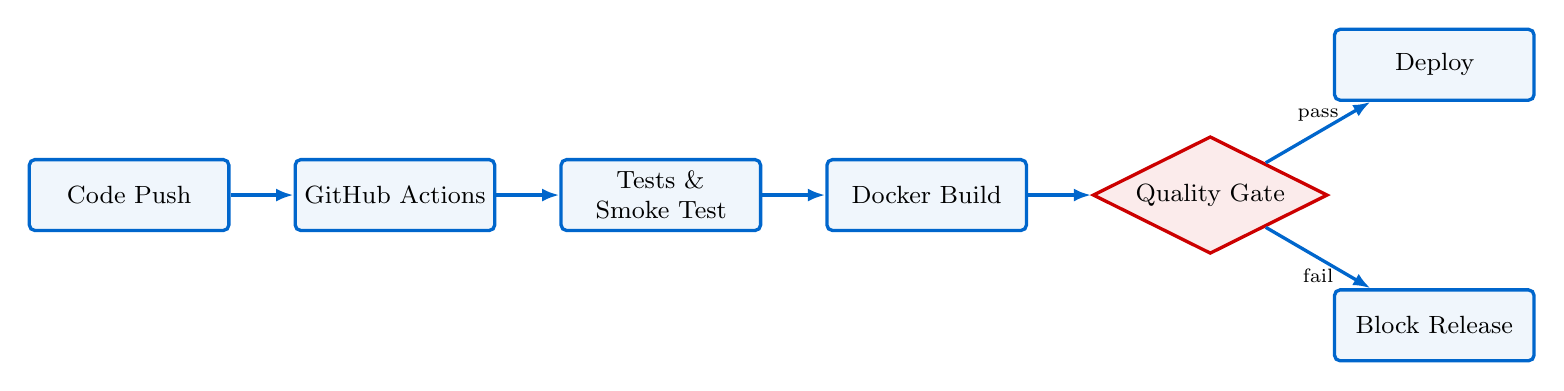
\begin{tikzpicture}[node distance=8mm and 8mm]
 \node[stage] (push) {Code Push};
 \node[stage, right=of push] (actions) {GitHub Actions};
 \node[stage, right=of actions] (tests) {Tests \& Smoke Test};
 \node[stage, right=of tests] (build) {Docker Build};
 \node[decision, right=of build] (gate) {Quality Gate};
 \node[stage, above right=of gate] (deploy) {Deploy};
 \node[stage, below right=of gate] (block) {Block Release};

 \draw[flowarrow] (push) -- (actions);
 \draw[flowarrow] (actions) -- (tests);
 \draw[flowarrow] (tests) -- (build);
 \draw[flowarrow] (build) -- (gate);
 \draw[flowarrow] (gate) -- node[above, font=\scriptsize] {pass} (deploy);
 \draw[flowarrow] (gate) -- node[below, font=\scriptsize] {fail} (block);
 \end{tikzpicture}%
 }
 \caption{Automated CI/CD workflow featuring cloud smoke testing and local Git hook triggers.}
\end{figure}

\subsection{Prefect Orchestration}
All machine learning tasks are orchestrated by Prefect. This ensures that data loading, training, and evaluation occur in a strict, observable sequence with automated retries and failure logging.

\begin{figure}[H]
 \centering
 \resizebox{\columnwidth}{!}{%
 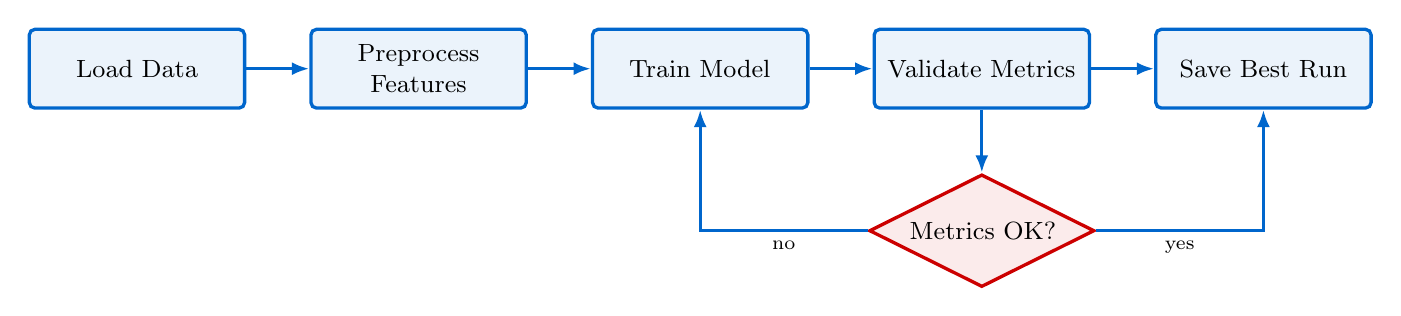
\begin{tikzpicture}[node distance=8mm and 8mm]
 \node[flowbox] (load) {Load Data};
 \node[flowbox, right=of load] (prep) {Preprocess Features};
 \node[flowbox, right=of prep] (train) {Train Model};
 \node[flowbox, right=of train] (validate) {Validate Metrics};
 \node[flowbox, right=of validate] (save) {Save Best Run};
 \node[decision, below=of validate] (retry) {Metrics OK?};

 \draw[flowarrow] (load) -- (prep);
 \draw[flowarrow] (prep) -- (train);
 \draw[flowarrow] (train) -- (validate);
 \draw[flowarrow] (validate) -- (save);
 \draw[flowarrow] (validate) -- (retry);
 \draw[flowarrow] (retry.west) -| node[pos=0.25, below, font=\scriptsize] {no} (train.south);
 \draw[flowarrow] (retry.east) -| node[pos=0.25, below, font=\scriptsize] {yes} (save.south);
 \end{tikzpicture}%
 }
 \caption{Prefect orchestration flow for model training and validation.}
\end{figure}

\section{Operational Notes and Future Work}
\subsection{How a Full Run Happens}
A full run starts by loading the CSV files, then the pipeline performs EDA on the raw data, trains the model, runs EDA again on the transformed data, evaluates the result, writes metrics to disk, and only then saves the model. That order is deliberate: it gives us visibility into both the starting data and the transformed features.

\begin{figure}[H]
 \centering
 \resizebox{\columnwidth}{!}{%
 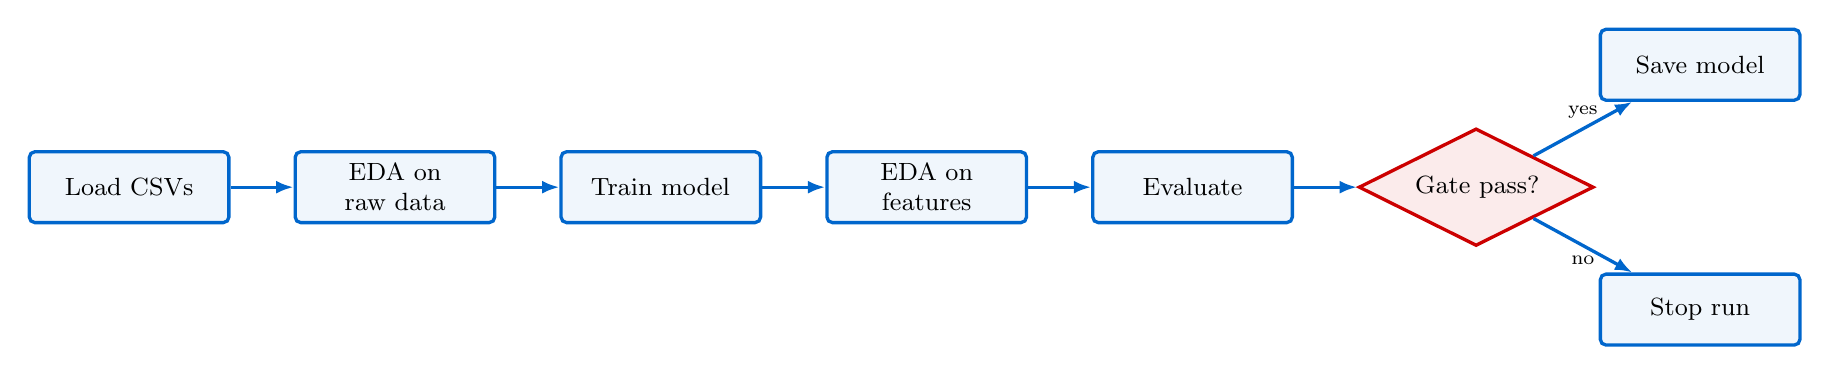
\begin{tikzpicture}[node distance=7mm and 8mm]
 \node[stage] (load) {Load CSVs};
 \node[stage, right=of load] (eda1) {EDA on raw data};
 \node[stage, right=of eda1] (train) {Train model};
 \node[stage, right=of train] (eda2) {EDA on features};
 \node[stage, right=of eda2] (eval) {Evaluate};
 \node[decision, right=of eval] (gate) {Gate pass?};
 \node[stage, above right=of gate] (save) {Save model};
 \node[stage, below right=of gate] (stop) {Stop run};
 \draw[flowarrow] (load) -- (eda1);
 \draw[flowarrow] (eda1) -- (train);
 \draw[flowarrow] (train) -- (eda2);
 \draw[flowarrow] (eda2) -- (eval);
 \draw[flowarrow] (eval) -- (gate);
 \draw[flowarrow] (gate) -- node[above, font=\scriptsize] {yes} (save);
 \draw[flowarrow] (gate) -- node[below, font=\scriptsize] {no} (stop);
 \end{tikzpicture}%
 }
 \caption{The end-to-end run order used by Prefect and the training pipeline.}
\end{figure}

\subsection{Monitoring and Model Health}
Beyond performance metrics, the pipeline incorporates automated drift detection using the **Evidently.ai** framework. This stage generates a comprehensive "Model Health Report" comparing the current training distribution against a historical baseline. It evaluates regression metrics, feature drift, and clustering stability, providing an early warning system for concept drift—a common failure mode in fraud detection where adversary behavior shifts over time.

\begin{table}[H]
\centering
\caption{Project components and their operational roles}
\begin{tabular}{p{0.22\columnwidth}p{0.32\columnwidth}p{0.28\columnwidth}}
\toprule
Component & Simple role & When it matters \\
\midrule
Prefect & Orchestrates task sequencing and error handling & During training and retraining \\
FastAPI & Serves low-latency predictions via HTTP & Real-time inference and UI interaction \\
Evidently & Automated drift and health reporting & Post-training validation and monitoring \\
Docker & Environment parity and microservice isolation & Deployment and CI/CD validation \\
Git Hooks & Local automation and instant feedback & Developer workflow and iteration \\
\bottomrule
\end{tabular}
\end{table}

\subsection{Future Work}
The next natural improvements are to add live drift monitoring, more robust probability calibration, and better integration between the dashboard and the latest model artifacts. Another useful step would be to add a richer explanation layer so an analyst can see which inputs pushed a prediction toward fraud.

\subsection{Final Observations and Future Work}
The project bridges research and production engineering by combining a measured modeling strategy with a fully operational serving stack. In practical terms, it shows that a carefully controlled tabular-learning pipeline can still perform strongly in a domain where the minority class is rare, feature redundancy is high, and the deployment environment must remain deterministic. The achieved ROC-AUC exceeds the paper benchmark, while the PR-AUC remains close to the target, confirming that the system is competitive rather than merely functional.

Future work will focus on:
\begin{itemize}
 \item Integrating **Real-Time Feature Stores** to reduce latency in user behavioral aggregates.
 \item Implementing **Graph Neural Networks (GNNs)** to capture network-level fraudulent relationships.
 \item Expanding the dashboard to include real-time drift monitoring and automated model retraining.
\end{itemize}

\end{document}
